\documentclass[aspectratio=169,t,xcolor=table]{beamer}
\usepackage[utf8]{inputenc}

\usepackage{booktabs} 
\usepackage{subcaption}

\usetheme{Ufg}

%-------------------------------------theorems--------------
\newtheorem{conj}{Conjetura}
\newtheorem{defi}{Definição}
\newtheorem{teo}{Teorema}
\newtheorem{lema}{Lema}
\newtheorem{prop}{Proposição}
\newtheorem{cor}{Corolário}
\newtheorem{ex}{Exemplo}
\newtheorem{exer}{Exercício}

\setbeamertemplate{theorems}[numbered]
\setbeamertemplate{caption}[numbered]

%-------------------------------------------------------------%
%----------------------- Primary Definitions -----------------%

% This command set the default Color, is also possible to choose a custom color
\setPrimaryColor{UFGBlue} 

% First one is logo in title slide (we recommend use a horizontal image), and second one is the logo used in the remaining slides (we recommend use a square image)
\setLogos{lib/logos/infw.png}{lib/logos/infw2.png} 


% -------------------------------------- Title Slide Information
\begin{document}
\title[Inf UFG]{SDSS: A Self-Supervised Spheroid Segmentation
Method}

\author{Guilherme V Leite\\ \bigskip Advisor: Hélio Pedrini}

\date{2022}
%-----------------------The next statement creates the title page.
\frame[noframenumbering]{\titlepage}


%------------------------------------------------Slide 1
\setLayout{vertical} % This command define the layout. 'vertical' can be replace with 'horizontal', 'blank, 'mainpoint', 'titlepage'

\begin{frame}[noframenumbering, plain]
    \frametitle{Table of Contents}
    \tableofcontents
\end{frame}

%---------------------------------------------------------
\section{Introduction}

% \setLayout{mainpoint}

\begin{frame}[noframenumbering, plain]{}
    \frametitle{Introduction}
\end{frame}

% \setLayout{vertical}

%---------------------------------------------------------
\begin{frame}
    \frametitle{Cell Cultures}
    \begin{columns}
        \column{0.5\textwidth}
            \begin{itemize}
                \item<1-> Vital to applications in:
                \begin{itemize}
                    \item<2-> Industry.
                    \item<3-> Academics.
                \end{itemize}
            \end{itemize}
            
                \begin{figure}[!htb]
                    \centering
                    \visible<6->{\subfloat{
\includegraphics[width=1.5cm]{figures/introduction/in_silico}} \hspace*{0.3cm}
                    \subfloat{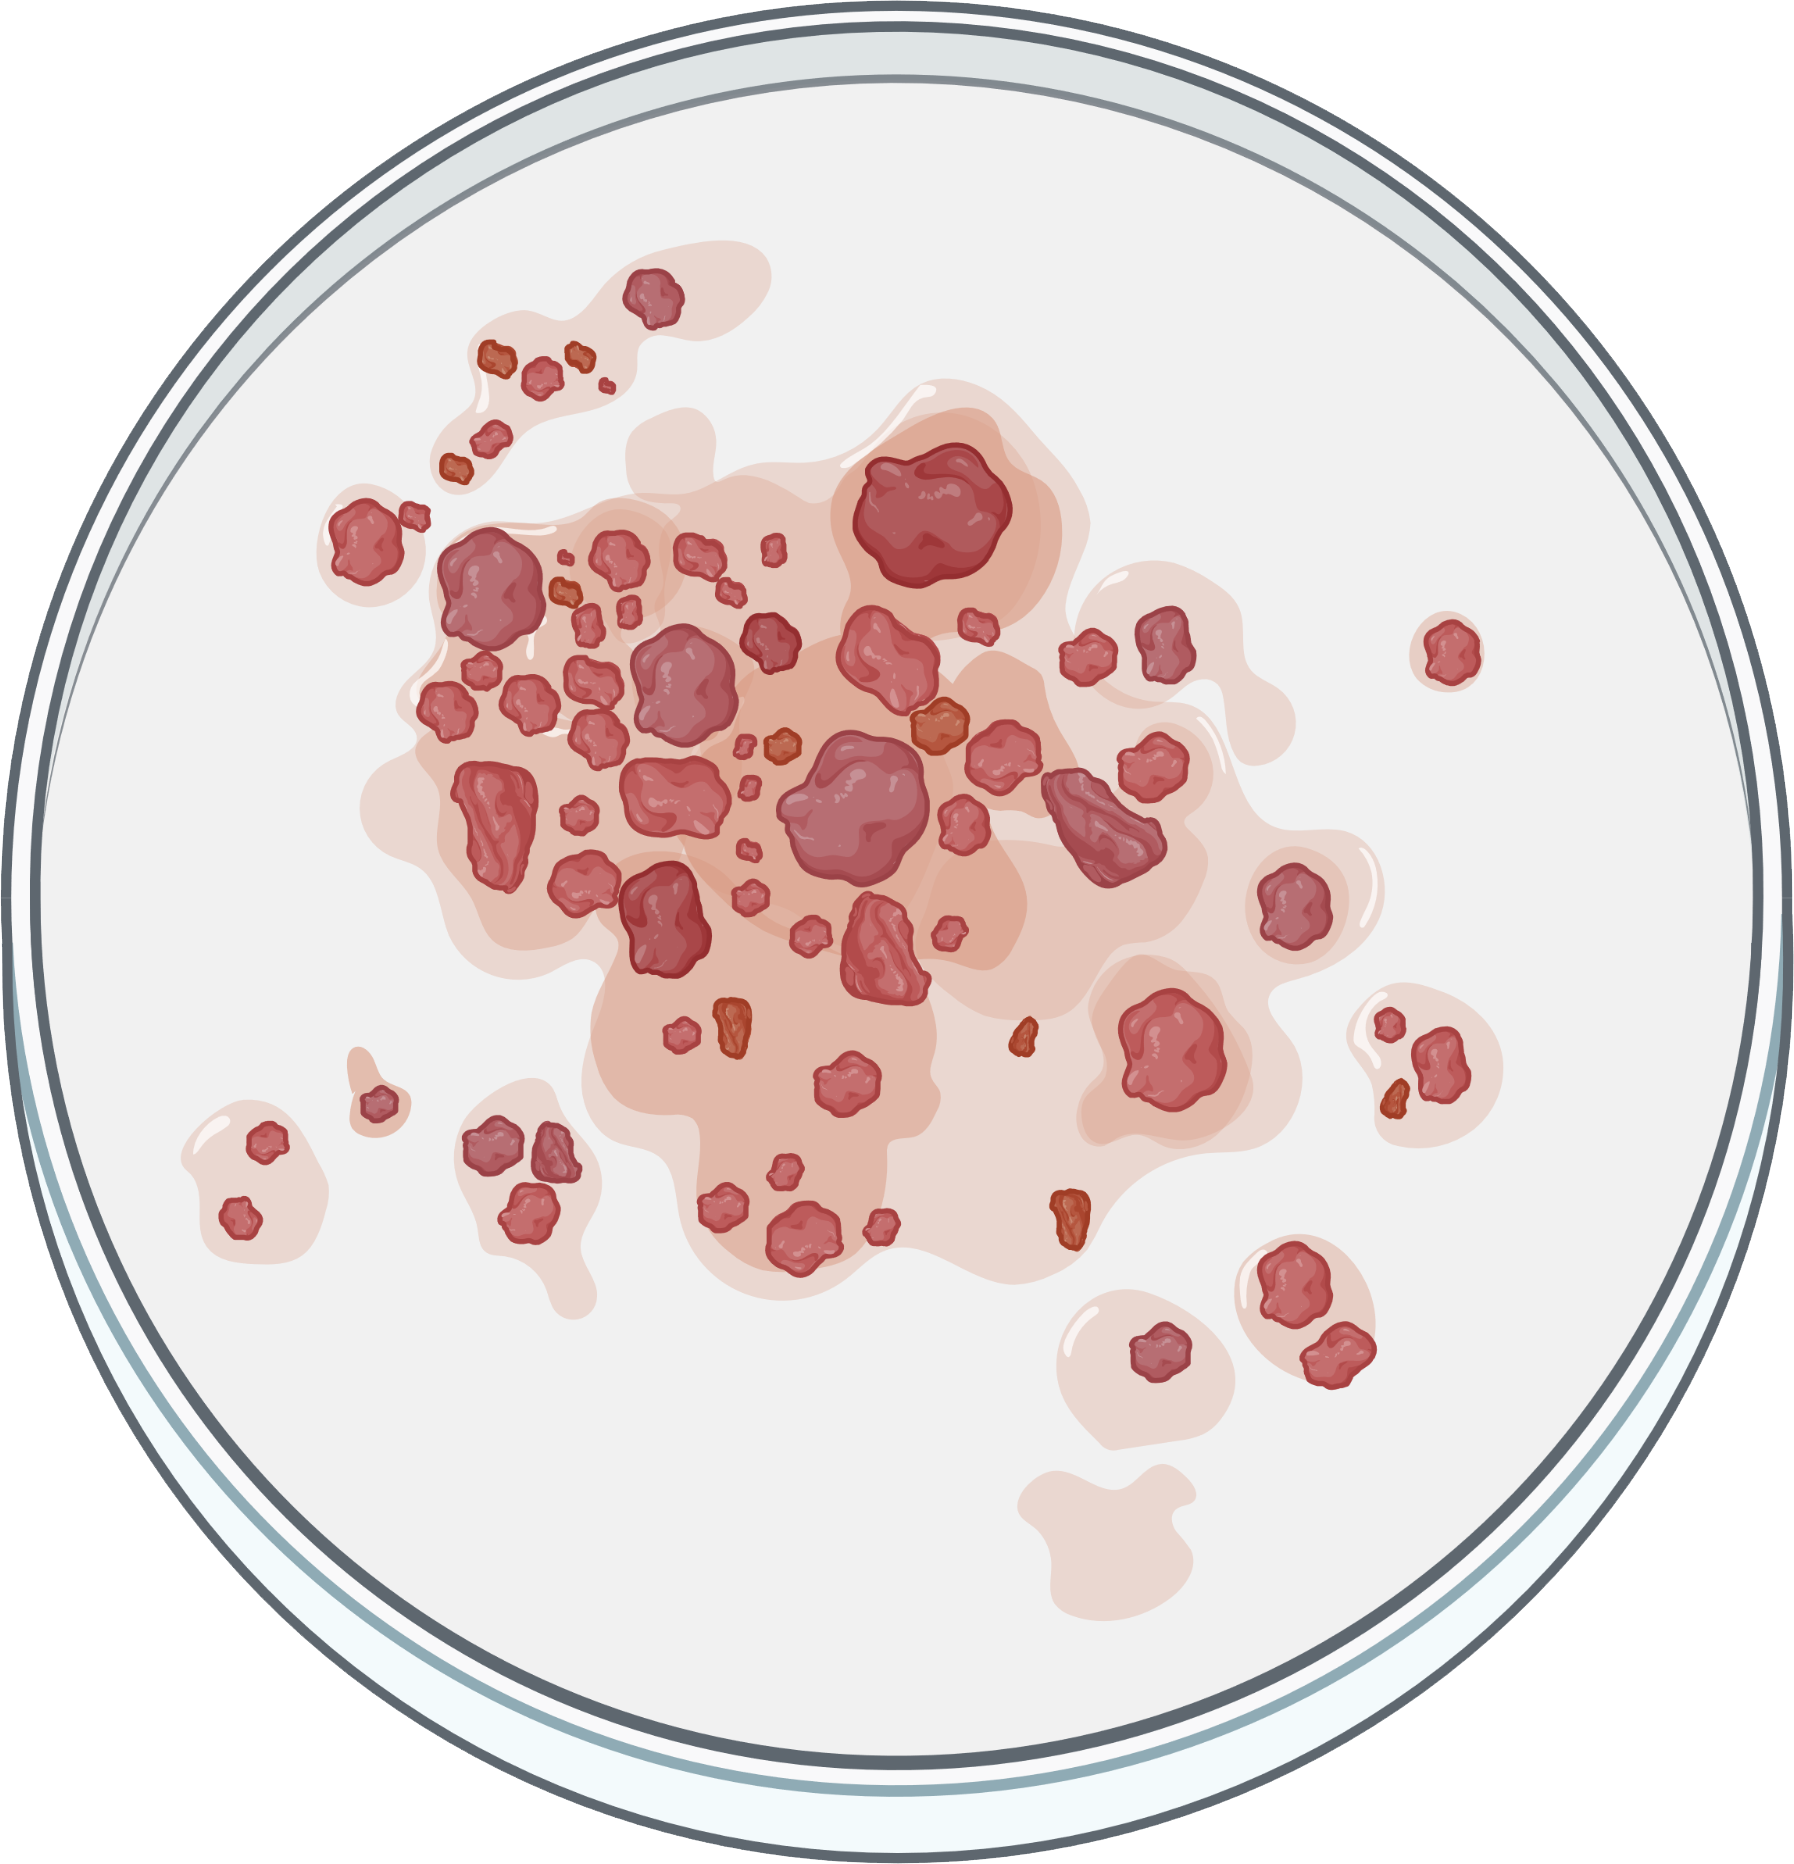
\includegraphics[width=1.5cm]{figures/introduction/in_vitro}} \hspace*{0.3cm}
                    \subfloat{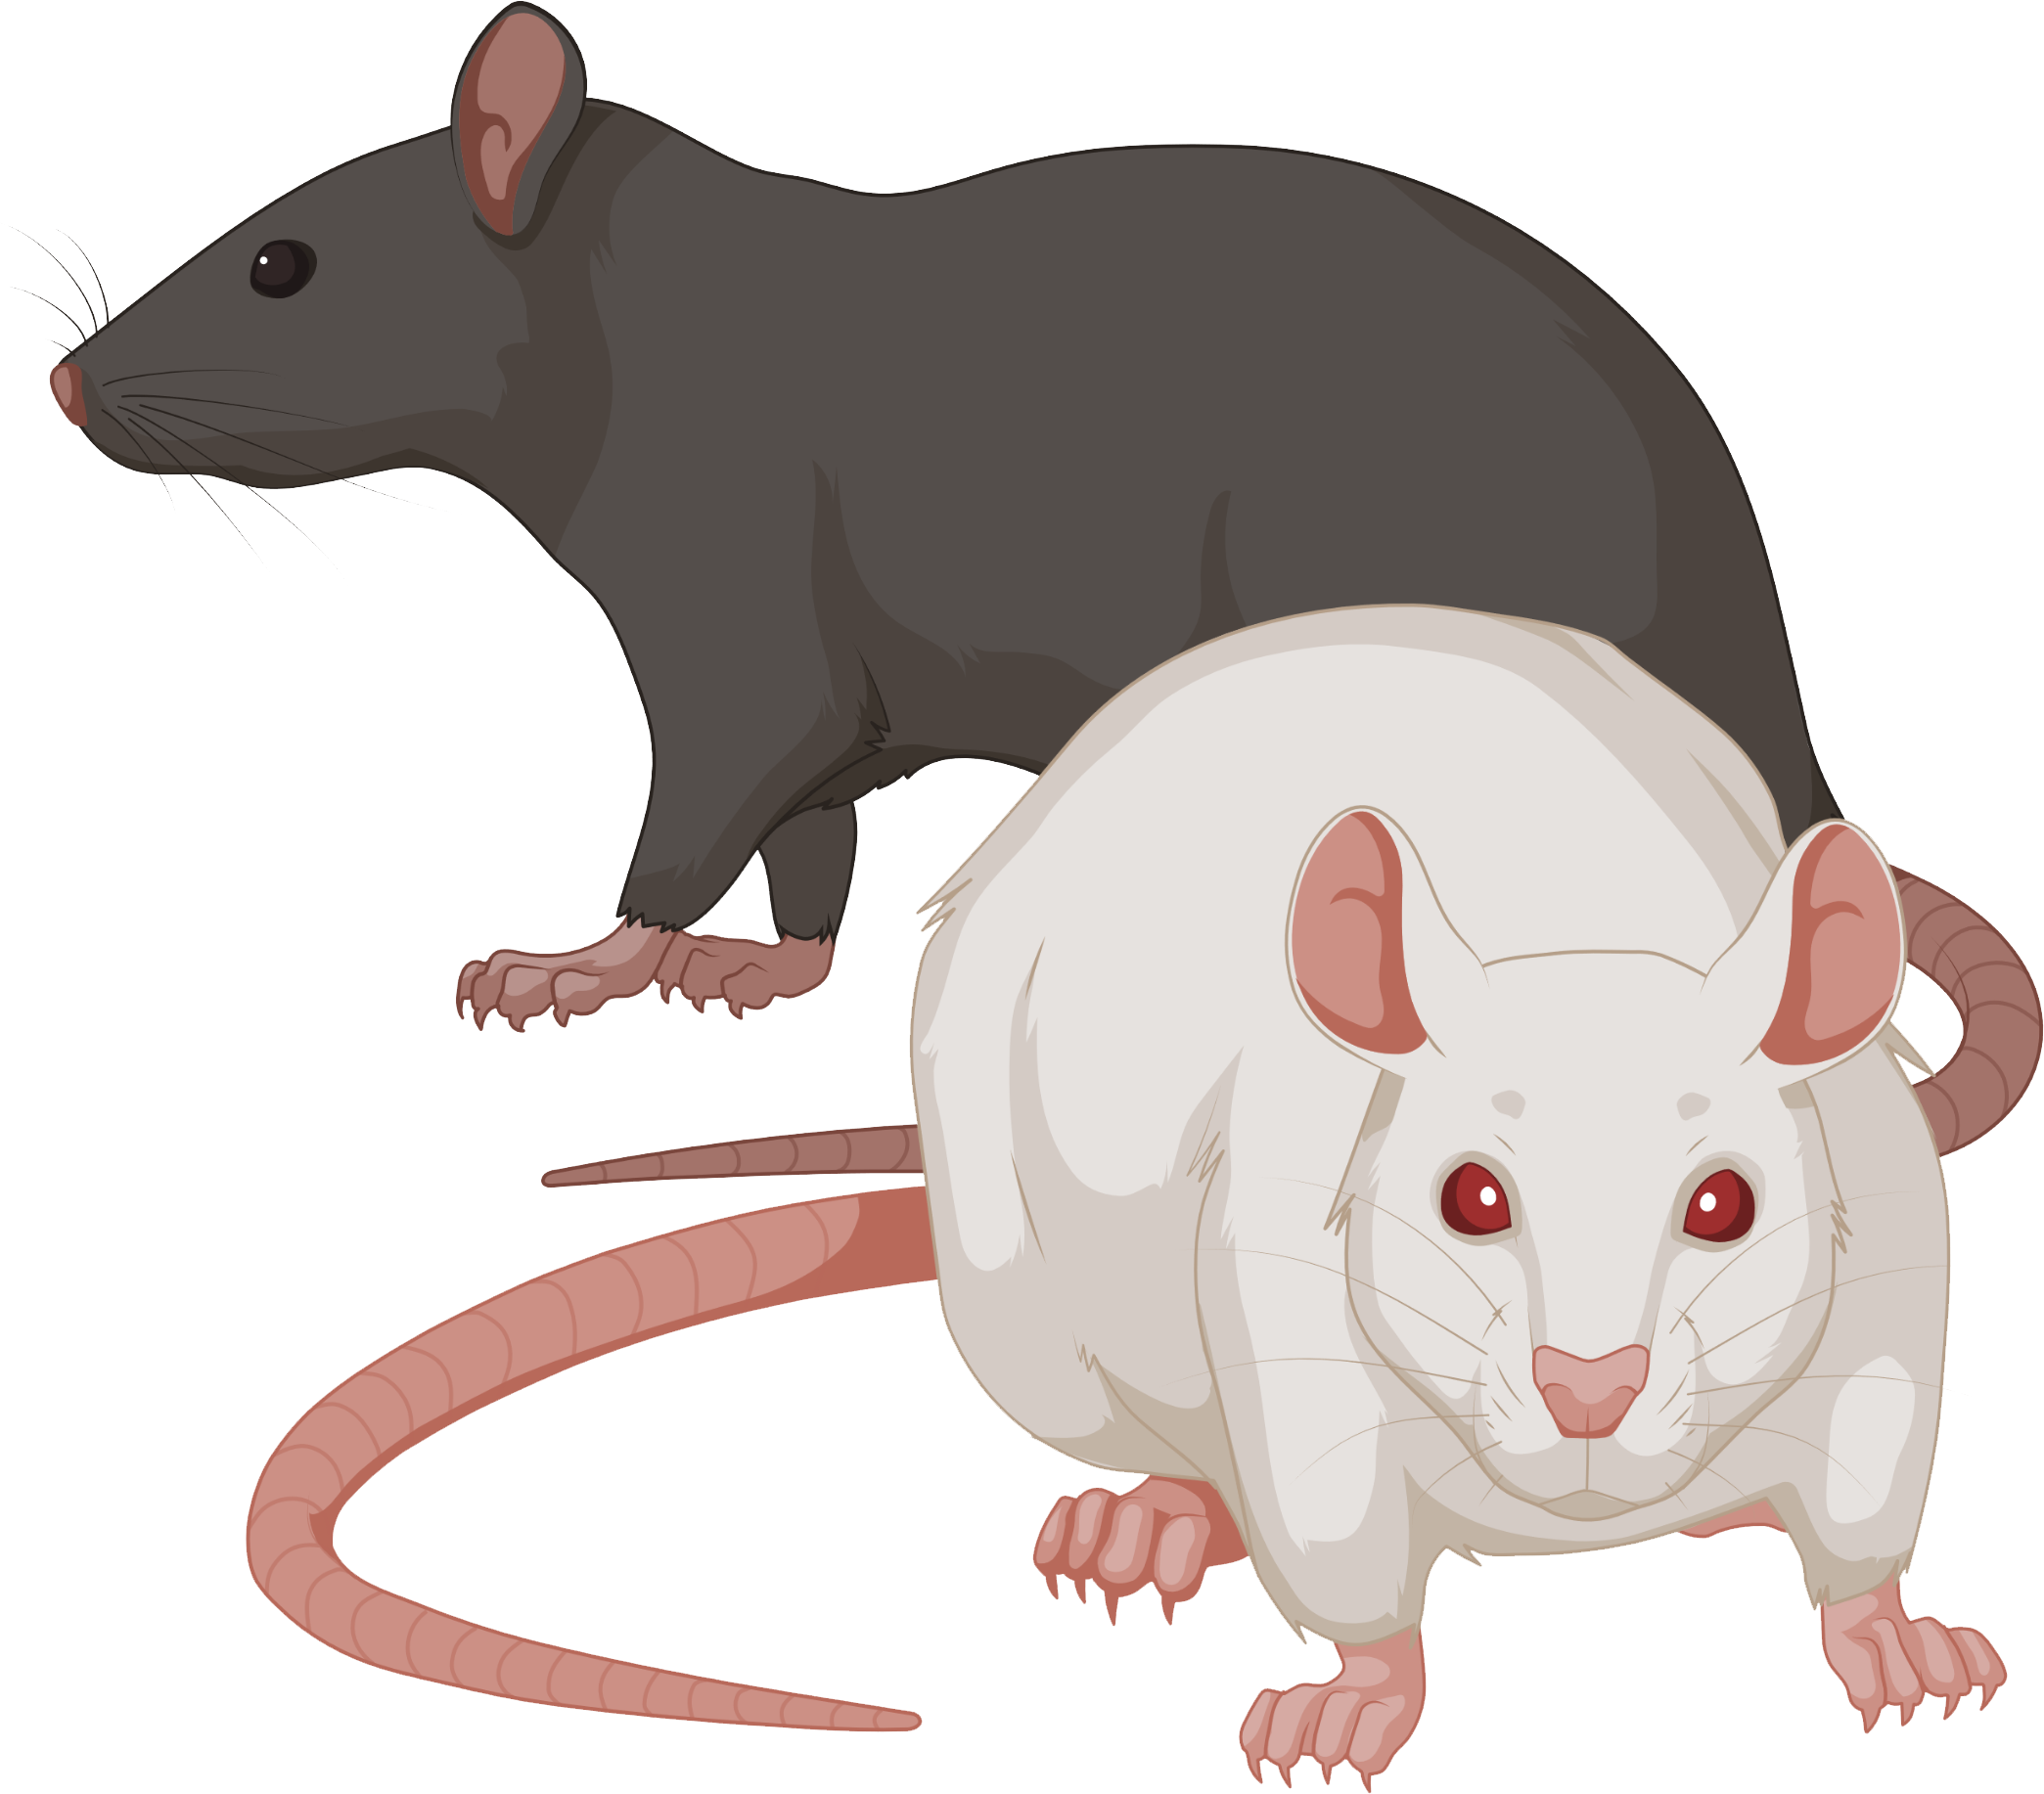
\includegraphics[width=1.5cm]{figures/introduction/in_vivo}}\\
                    Pre-Clinical}
                    \visible<7->{\subfloat{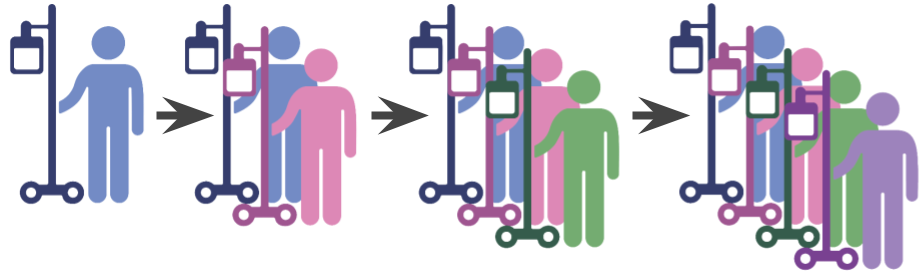
\includegraphics[width=5cm]{figures/introduction/clinical}}\\
                    Clinical}
                \end{figure}
        \column{0.5\textwidth}
            \begin{itemize}    
                \item<4-> Pharmaceutical context:
                    \begin{itemize}
                        \item<5-> Drug discovery and development.
                        \begin{itemize}
                            \item<6-> Pre-Clinical.
                            \item<7-> Clinical trials.
                        \end{itemize}
                    \end{itemize}
            \end{itemize}
    \end{columns}
\end{frame}

%---------------------------------------------------------
\begin{frame}{Drug Discovery}
    \begin{figure}[!htb]
    \centering
    \setbeamercovered{transparent}
    \visible<1->{\subfloat[\textit{in silico}]{
\includegraphics[width=2cm]{figures/introduction/in_silico}} \hspace*{0.3cm}}
    \visible<2->{\subfloat[\textit{in vitro}]{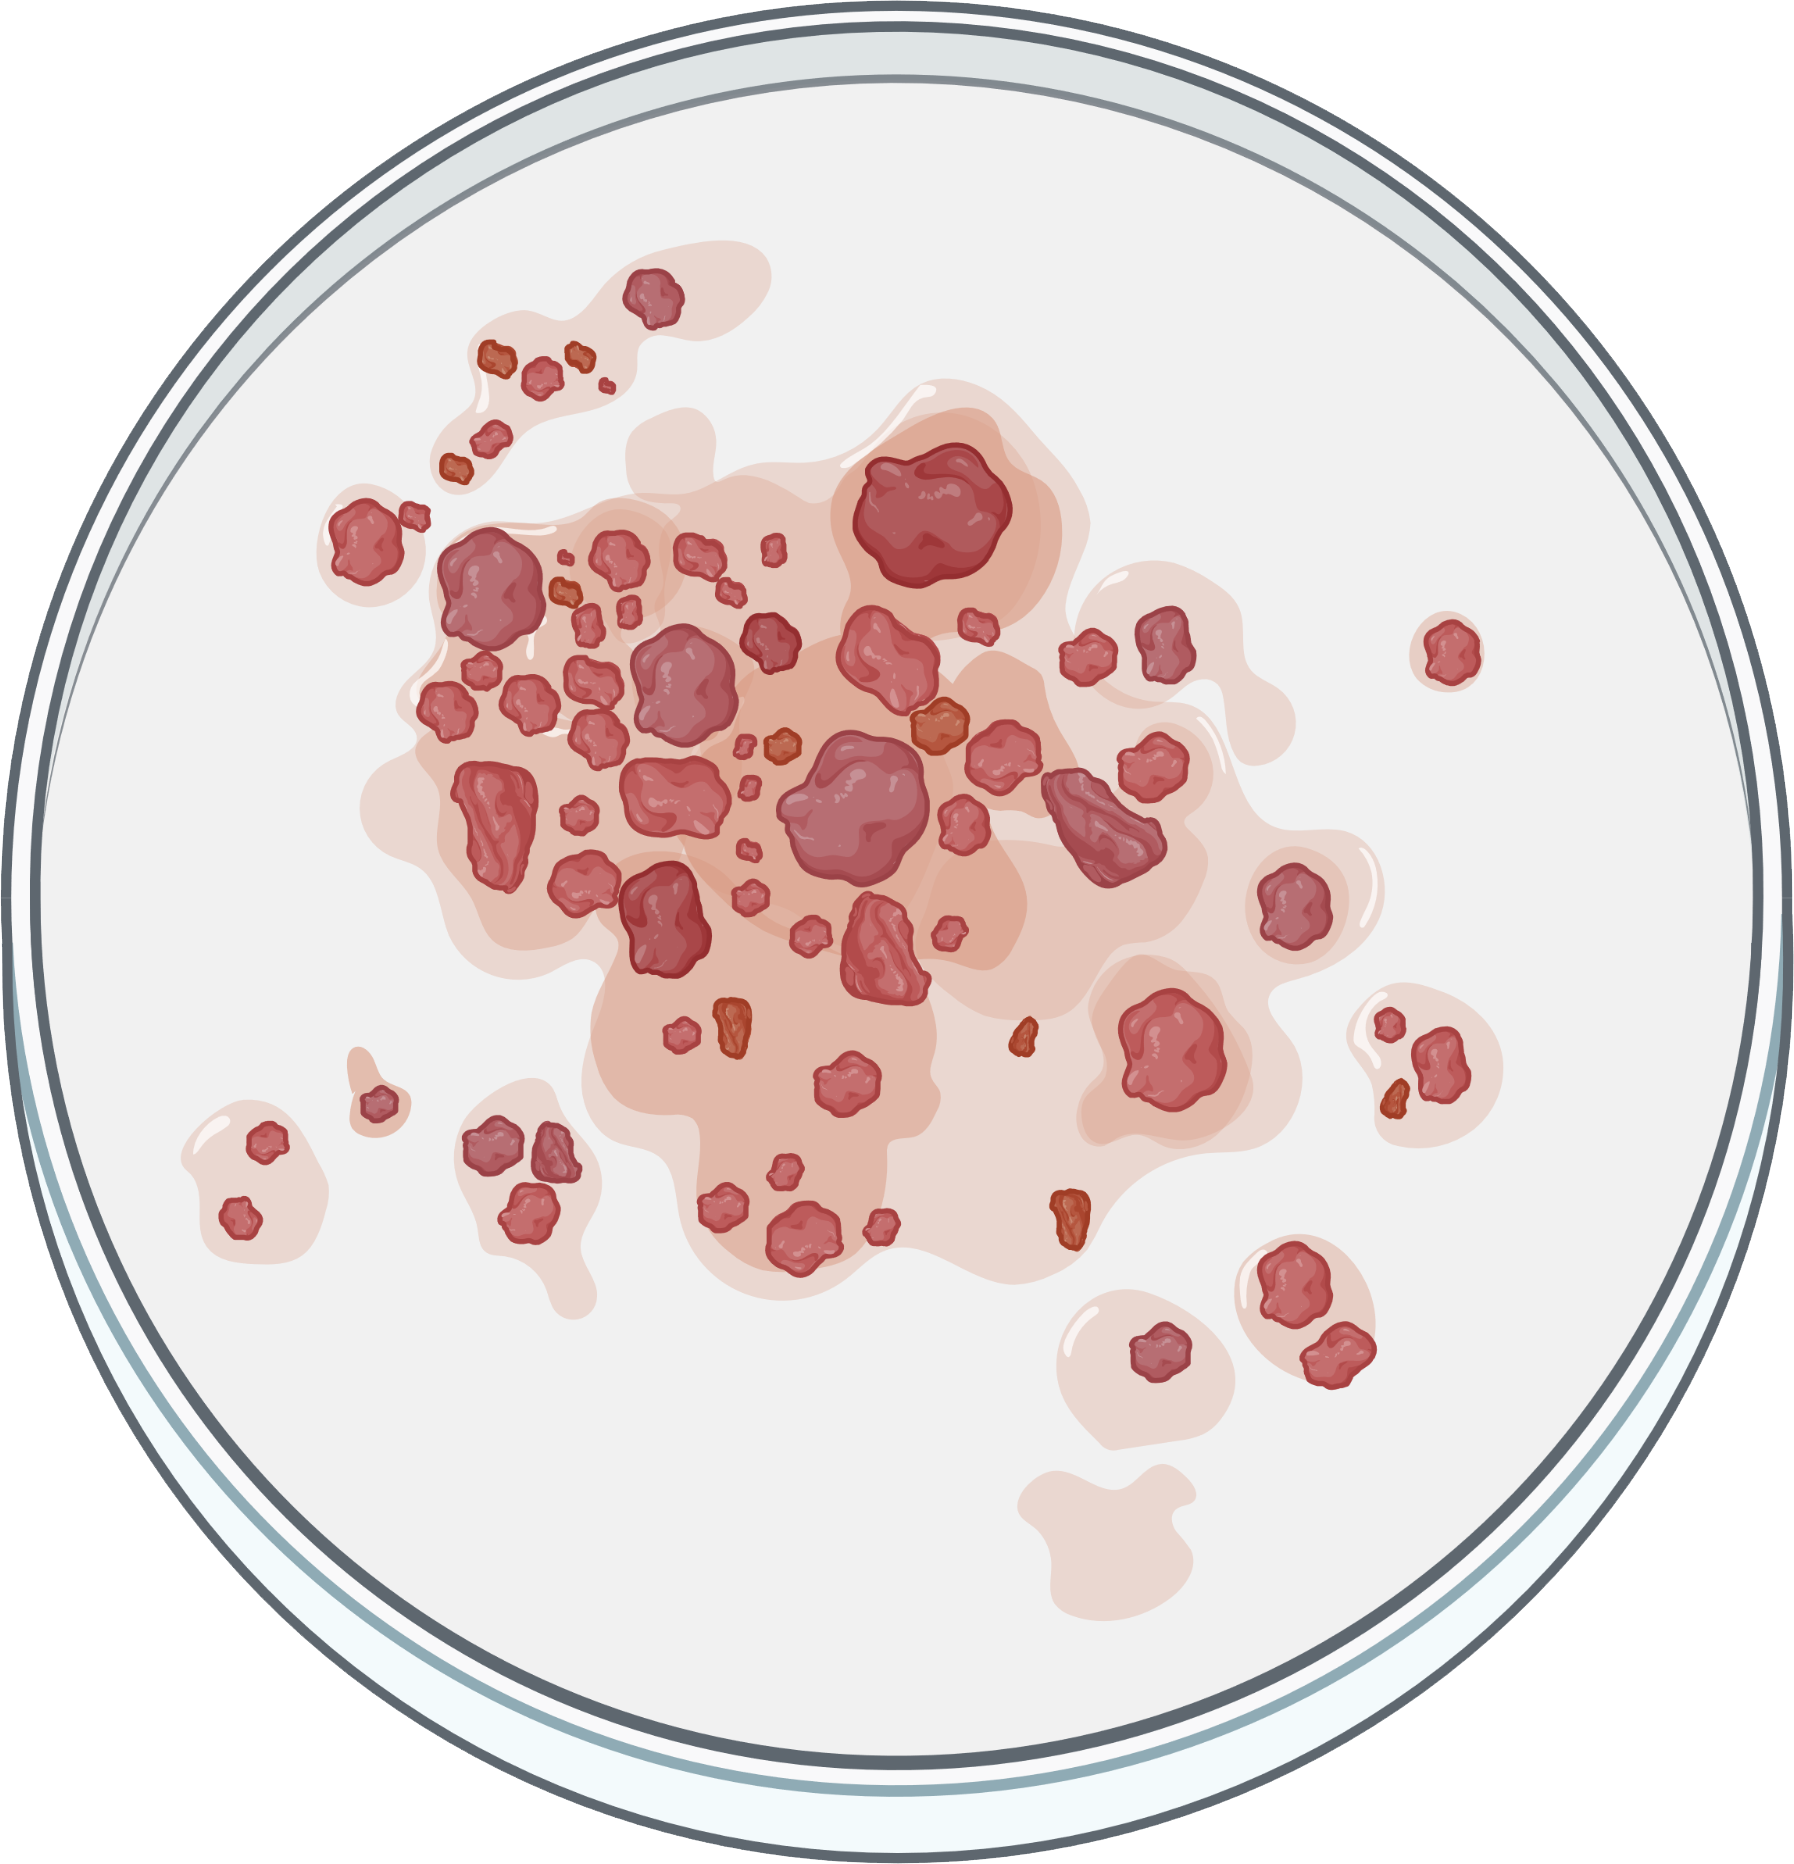
\includegraphics[width=2cm]{figures/introduction/in_vitro}} \hspace*{0.3cm}}
    \visible<3->{\subfloat[\textit{in vivo}]{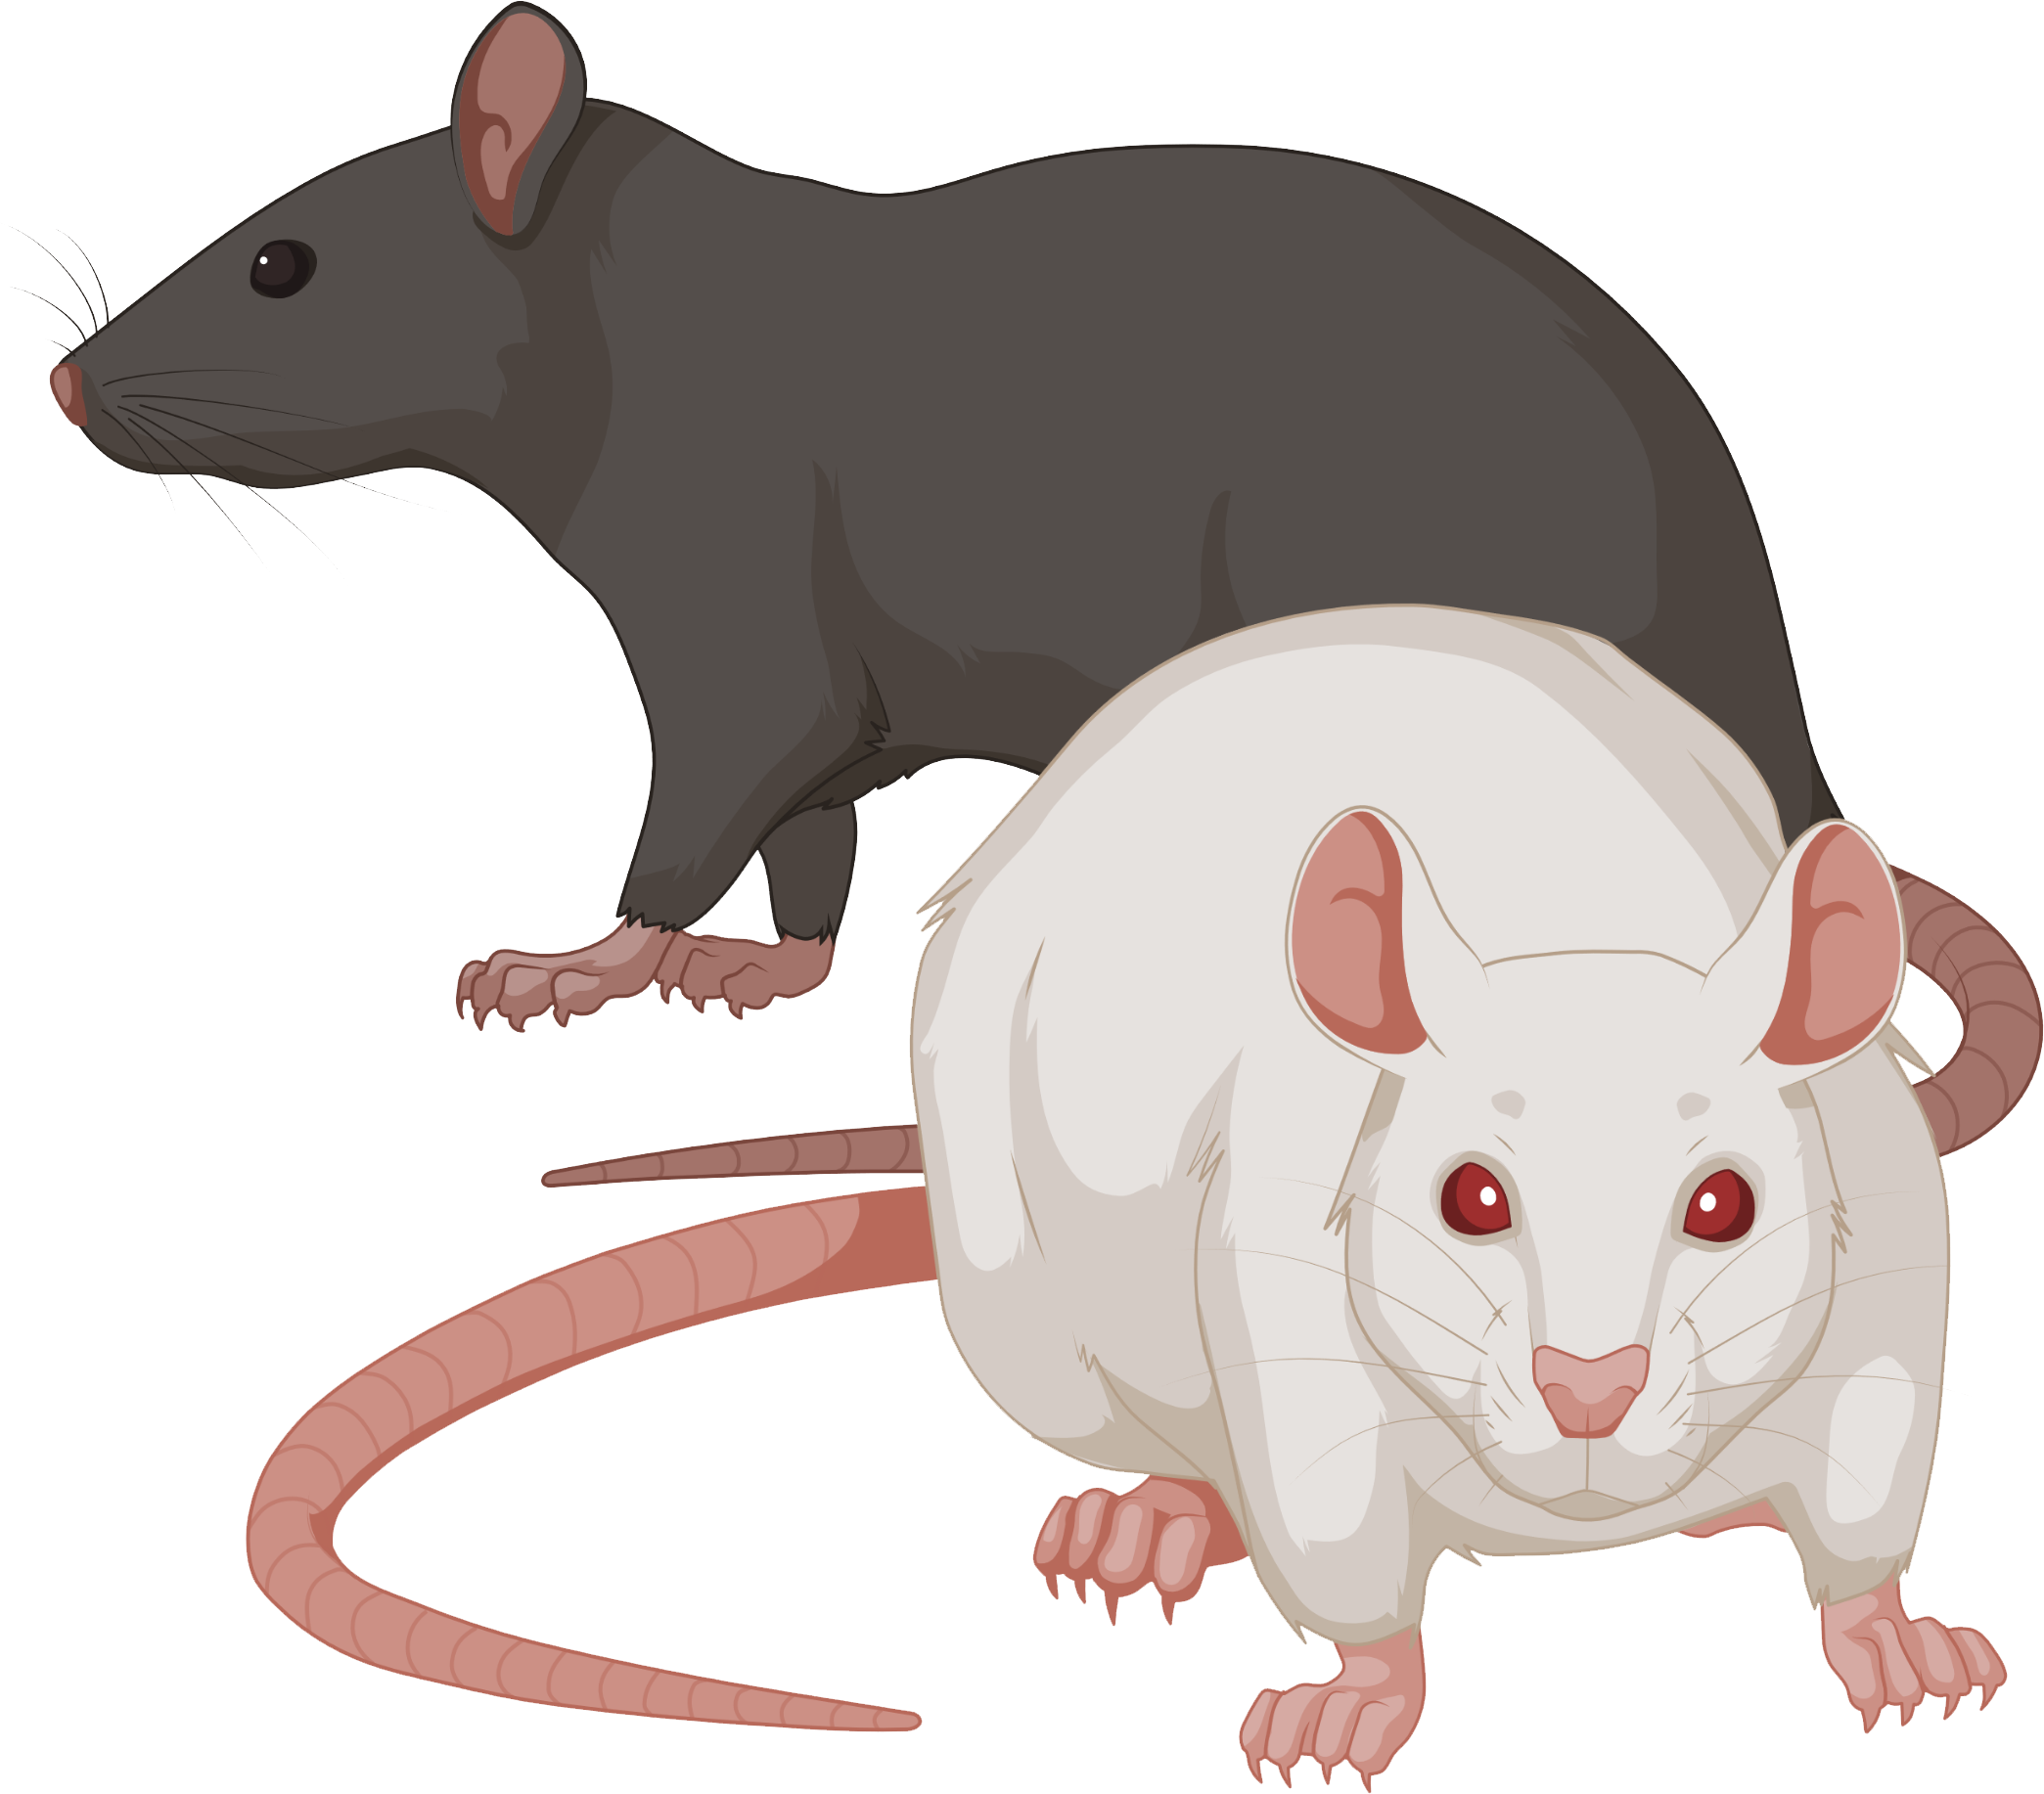
\includegraphics[width=2cm]{figures/introduction/in_vivo}}}\\
    \visible<4->{\subfloat[Clinical Trials]{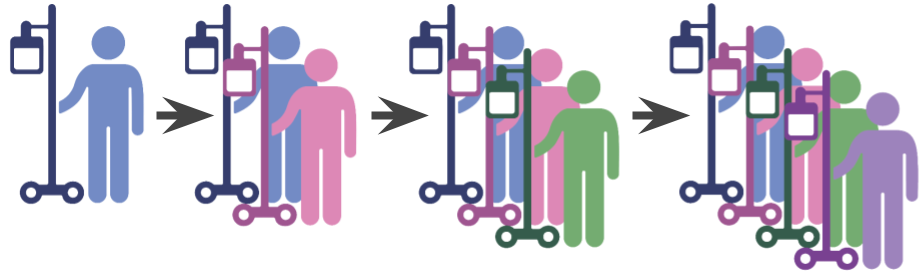
\includegraphics[width=9cm]{figures/introduction/clinical}}}
    \end{figure}
\end{frame}

%---------------------------------------------------------
\begin{frame}{Drug Discovery}
    \begin{columns}
        \column{0.4\textwidth}
            \begin{itemize}
                \item<1-> This process is:
                \begin{itemize}
                    \item<2-> Laborious.
                    \item<3-> Expensive.
                    \item<4-> Time consuming.
                \end{itemize}
                \item<5-> Low success rate:
                \begin{itemize}
                    \item<6-> Only \alert{10\%} moves to clinical trials.
                \end{itemize}
            \end{itemize}
        \column{0.4\textwidth}
            \begin{itemize}
                \item<7-> Fails are attributed to \alert{pre-clinical} stages.
                \begin{itemize}
                    \item<8-> Too simple.
                    \item<9-> Failed to eliminate bad candidates.
                \end{itemize}
            \end{itemize}
    \end{columns}
\end{frame}

%---------------------------------------------------------
\begin{frame}{2D Cultures}
    \begin{columns}
        \column{0.45\textwidth}
        \begin{itemize}
            \item<1-> Most common culture.
            \item<2-> Cells grow:
            \begin{itemize}
                \item<3-> In the culture medium.
                \item<4-> Monolayer.
                \item<5-> Attached to the substrate.
            \end{itemize}
        \end{itemize}

        \begin{figure}[!htb]
            \centering
            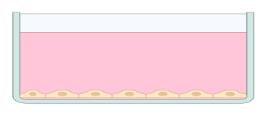
\includegraphics[width=6cm]{figures/introduction/2D_culture}
        \end{figure}

        \column{0.5\textwidth}
        \begin{itemize}
            \item<6-> Practical to evaluate compounds, since:
            \begin{itemize}
                \item<7-> No ethical committee required.
                \item<8-> Widespread training of personnel.
                \item<9-> Immortalized cells.
                \item<10-> Cells are genetically similar.
                \item<11-> Cells can be frozen.
                \item<12-> Cheaper upkeep.
            \end{itemize}
            \item<13-> Downside:
                \begin{itemize}
                    \item<14-> Can't reproduce microenvironment.
                \end{itemize}
        \end{itemize}
    \end{columns}
\end{frame}

%---------------------------------------------------------
\begin{frame}{3D Cultures}
    \begin{columns}
        \column{0.45\textwidth}
        \begin{figure}[!htb]
            \centering
            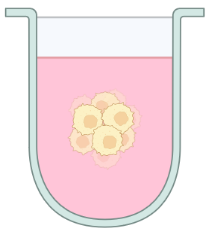
\includegraphics[width=6cm]{figures/introduction/3D_culture}
        \end{figure}

        \column{0.5\textwidth}
        \begin{itemize}
            \item<1-> Cells grow:
                \begin{itemize}
                    \item<1-> Floating in the culture medium.
                    \item<2-> With or without scaffolding.
                \end{itemize}
            \item<3-> Microenvironment reproduction:
            \begin{itemize}
                \item<4-> Cell-to-cell communication.
                \item<5-> Interactions between stroma and cell.
                \item<6-> Cell differentiation.
            \end{itemize}
            \item<7-> Better \textit{in vitro} alternative:
            \begin{itemize}
                \item<8-> Faster testing.
                \item<9-> Automation.
                \item<10-> Reproducibility.
            \end{itemize}
        \end{itemize}
    \end{columns}
\end{frame}

%---------------------------------------------------------
\begin{frame}{Spheroid Regions}
    \begin{figure}
        \centering
        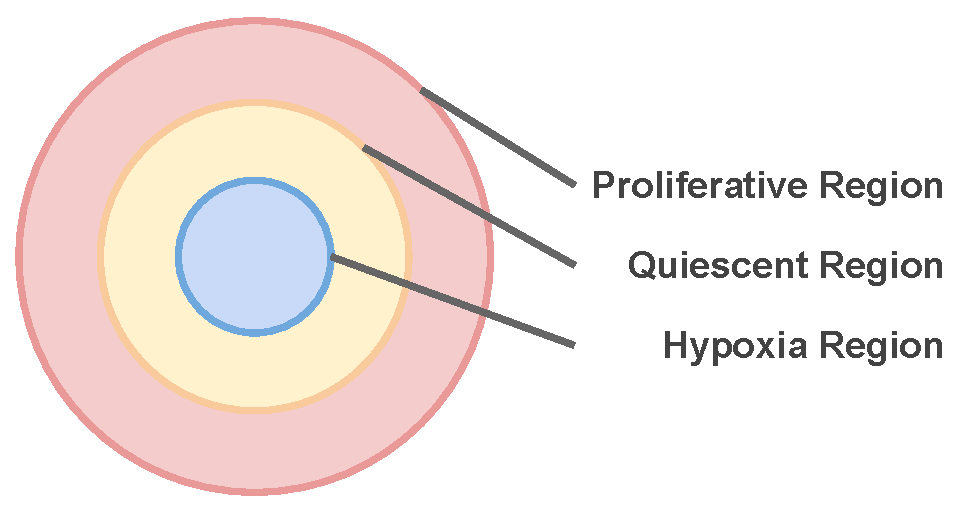
\includegraphics[width=8cm]{figures/introduction/spheroid_regions}
        \label{fig:spheroid_regions}
    \end{figure}
\end{frame}

%---------------------------------------------------------
\begin{frame}{Research Questions}
        \begin{enumerate}
            \item<1-> Shape-aware loss function \alert{affects} segmentation?
            \item<2-> Is the U-net encoder a \alert{better} generator backbone for spheroid segmentation?
            \item<3-> Can we evaluate spheroids with \alert{affected} proliferative zones?
            \item<4-> Is \alert{scale} important in spheroid segmentation?
            \item<5-> Can a single GAN differentiate \alert{all three} spheroid zones?
        \end{enumerate}
\end{frame}

%---------------------------------------------------------
% \setLayout{horizontal}

\begin{frame}{Objectives}
            \begin{block}{Global Objectives}
                \begin{columns}
                \column{0.5\textwidth}
                \begin{enumerate}
                    \item Create the spheroid image\\ dataset (SDSS).
                \end{enumerate}
                \column{0.5\textwidth}
                \begin{enumerate}
                \setcounter{enumi}{1}
                    \item A self-supervised semantic segmentation method.
                \end{enumerate}
                \end{columns}
            \end{block}
            \begin{block}{Specific Objectives}
                \begin{columns}
                \column{0.5\textwidth}
                \begin{enumerate}
                    \item Literature review.
                    \item Setup dataset.
                    \item Select metric.
                    \item Develop method.
                    \item Evaluate Loss functions.
                \end{enumerate}
                \column{0.5\textwidth}
                \begin{enumerate}
                \setcounter{enumi}{5}
                    \item Select GAN backbones.
                    \item Process results.
                \end{enumerate}
                \end{columns}
            \end{block}
\end{frame}

%---------------------------------------------------------
% \setLayout{vertical}

\begin{frame}{Expected Challenges}
    \begin{itemize}
        \item Access to data.
        \item Lack of protocols.
        \item Heterogeneous evaluation metrics.
        \item GANs convergence.
        \item Annotate images.
        \item Train with few samples.
    \end{itemize}
\end{frame}

%---------------------------------------------------------
\begin{frame}{Expected Contributions}
    \begin{itemize}
        \item New public dataset.
        \item New self-supervised segmentation method.
        \item Segmentation as an analysis tool.
        \item Qualitative study.
        \item Competitive results.
    \end{itemize}
\end{frame}
\begin{frame}{Expected Contributions}
    \begin{itemize}
        \item New public dataset.
        \item New self-supervised segmentation method.
        \item Segmentation as an analysis tool.
        \item Qualitative study.
        \item Competitive results.
    \end{itemize}
\end{frame}
\begin{frame}{Expected Contributions}
    \begin{itemize}
        \item New public dataset.
        \item New self-supervised segmentation method.
        \item Segmentation as an analysis tool.
        \item Qualitative study.
        \item Competitive results.
    \end{itemize}
\end{frame}

\setBGColor{Ocean}
\section{Related Literature}

\setLayout{mainpoint}

\begin{frame}[noframenumbering, plain]{}
    \frametitle{Related Literature}
\end{frame}

\setLayout{vertical}

%---------------------------------------------------------
\begin{frame}{Related Literature}
    \begin{table}
        \centering
        \setlength{\tabcolsep}{10pt}

        \rowcolors{2}{}{LightGray!10}
        \begin{tabular}{lrlr}
            \textbf{Authors} & \textbf{Method} & \textbf{Metric} & \textbf{Dataset} \\
            \toprule
            Lacalle et al. & DeepLabV3+ & $0.97$ Jaccard & \textbf{Public} \\
            Wen et al. & 3D U-Net & $0.97$ Accuracy & Private \\
            Vaidyanathan et al. & Custom & $0.95$ Dice & Private \\
            García-Domínguez et al. & $\mathrm{U}^2$-Net & $0.95$ Jaccard & Lacalle's \\
            Chen et al. & PSP-U-Net & $0.95$ F1-score & Private \\
            Ahmad et al. & U-Net$^*$ & $0.86$ F-score & Private \\
            Sadanandan et al. & GAN & $0.77$ maF & Private \\
            Grexa et al. & Mask R-CNN & $0.76$ AP & Request \\
            Aida et al. & CGAN & $0.10$ F-score & Private \\
            \midrule
            Choudhry et al. & Handcrafted & $0.99$ $R^2$ & Private \\
            Wenzel et al. & MetaXpress & - & Private \\
        \end{tabular}
    \end{table}
\end{frame}

%---------------------------------------------------------
\begin{frame}{Literature Limitations}
    \begin{itemize}
        \item Lack of public spheroid datasets.
        \item Handcrafted features.
    \end{itemize}
\end{frame}

\setBGColor{LightGreen}
\section{Datasets}

\setLayout{mainpoint}

\begin{frame}[noframenumbering, plain]{}
    \frametitle{Datasets}
\end{frame}

\setLayout{vertical}

%---------------------------------------------------------
\begin{frame}{Available Datasets}

    \begin{itemize}
        \item Majority of related works acquired their own images.
        \item The work of Lacalle et al.
    \end{itemize}

    \begin{table}[]
        \centering
        \setlength{\tabcolsep}{10pt}
        
        {\rowcolors{2}{}{LightGray!10}
            \begin{tabular}{lcccccc}
                \textbf{Name} & \textbf{BL5S} & \textbf{BN2S} & \textbf{BN10S} & \textbf{FL5C} & \textbf{FL5S} & \textbf{FN2S} \\
                \midrule
                Method & Brif & Brif & Brif & Fluo & Fluo & Fluo \\
                Images & 50 & 154 & 105 & 19 & 50 & 34 \\
                Magnification & 5x & 2x & 10x & 5x & 5x & 2x \\
                Culture & Susp & Susp & Susp & Colla & Susp & Susp
            \end{tabular}
        }
    \end{table}
\end{frame}

%---------------------------------------------------------
\begin{frame}{Lacalle et al. annotations}
   \begin{itemize}
       \item Annotated via ImageJ software.
       \item ImageJ only saves the vertices.
       \item Python script to generate mask images.
   \end{itemize}
\end{frame}

%---------------------------------------------------------
\begin{frame}{Samples from Lacalle et al.}
    \begin{figure}[!htb]
        \centering
        \subfloat{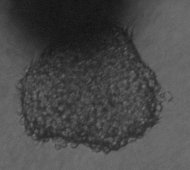
\includegraphics[width=3cm, height=3cm]{figures/datasets/1}}
        \subfloat{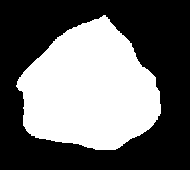
\includegraphics[width=3cm, height=3cm]{figures/datasets/1_mask}}\hspace*{0.1cm}
        \subfloat{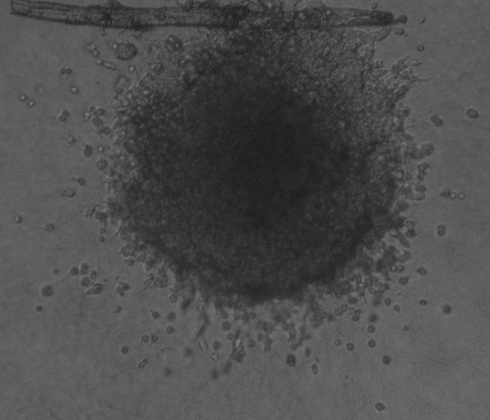
\includegraphics[width=3cm, height=3cm]{figures/datasets/11}}
        \subfloat{
\includegraphics[width=3cm, height=3cm]{figures/datasets/11_mask}}\\
        \subfloat{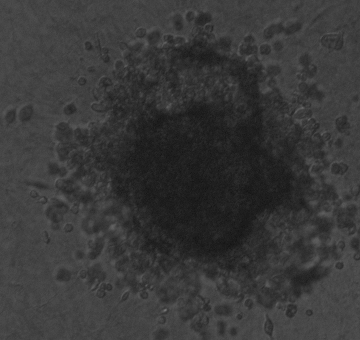
\includegraphics[width=3cm, height=3cm]{figures/datasets/7}}
        \subfloat{
\includegraphics[width=3cm, height=3cm]{figures/datasets/7_mask}}\hspace*{0.1cm}
        \subfloat{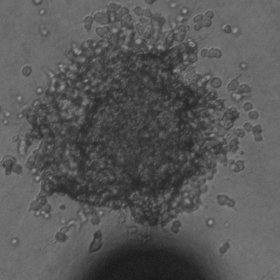
\includegraphics[width=3cm, height=3cm]{figures/datasets/6}}
        \subfloat{
\includegraphics[width=3cm, height=3cm]{figures/datasets/6_mask}}
    \end{figure}
\end{frame}

%---------------------------------------------------------
\begin{frame}{Proposed Datasets}
    \begin{itemize}
        \item OncoBiomarkers Research Laboratory at UNICAMP;
            %\begin{itemize}
                %\item Professor Carmen Veríssima Ferreira;
            %\end{itemize}
        \item Two images per spheroid;
    \end{itemize}
\end{frame}

%---------------------------------------------------------
\setLayout{horizontal}

\begin{frame}{Spheroid Acquisition}
    \begin{figure}[!htb]
        \centering
        \subfloat{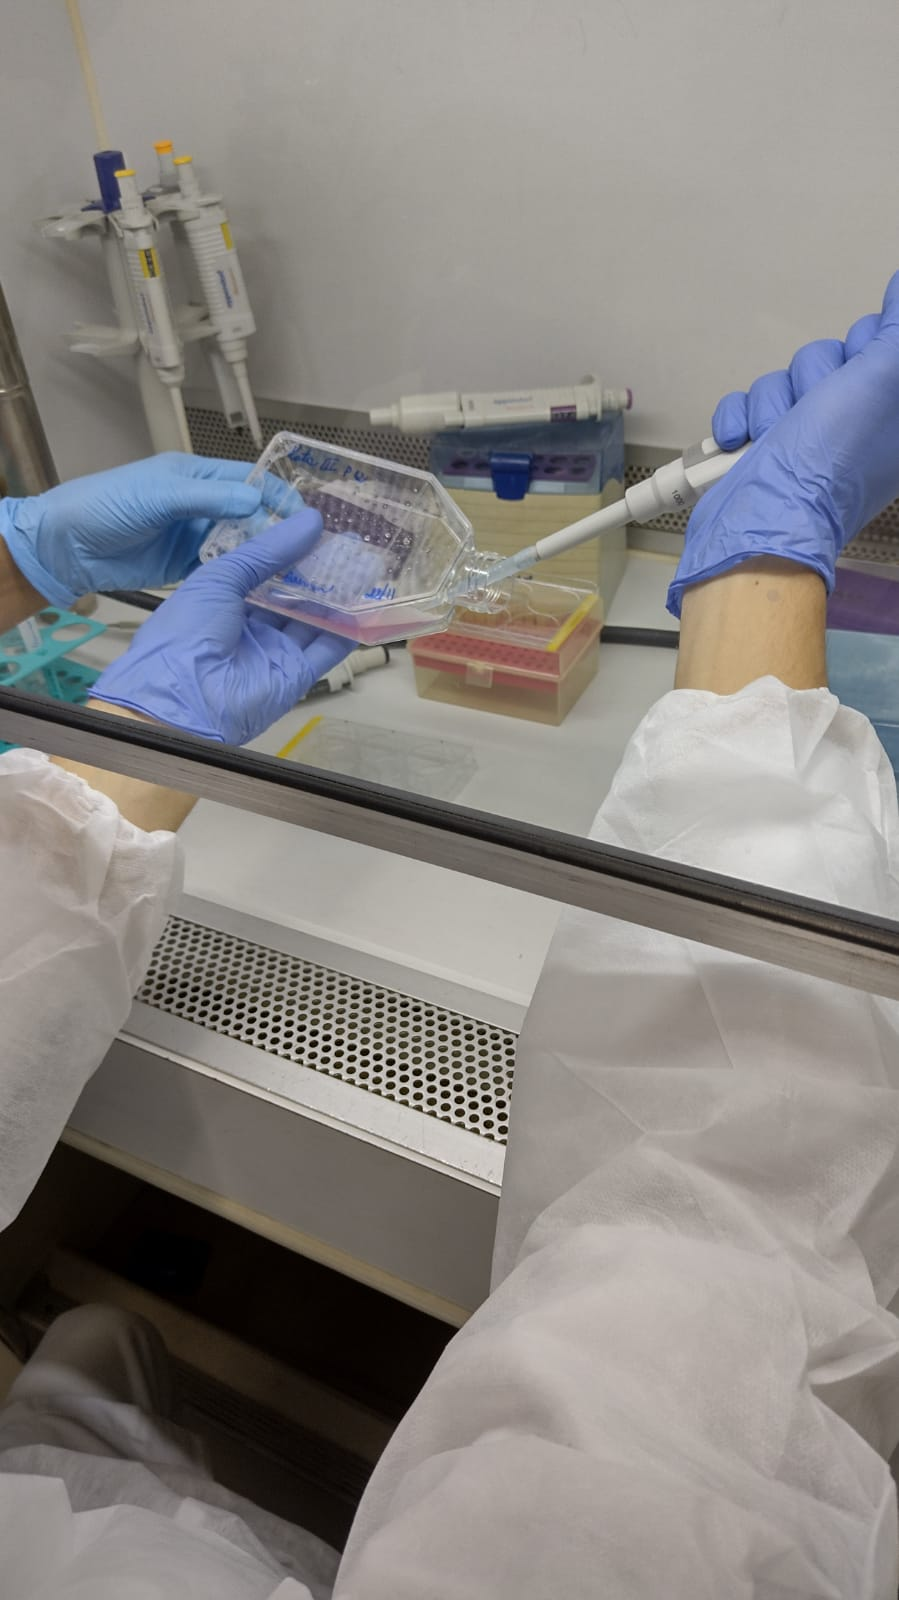
\includegraphics[width=2cm]{figures/datasets/spheroid_1}}
        \subfloat{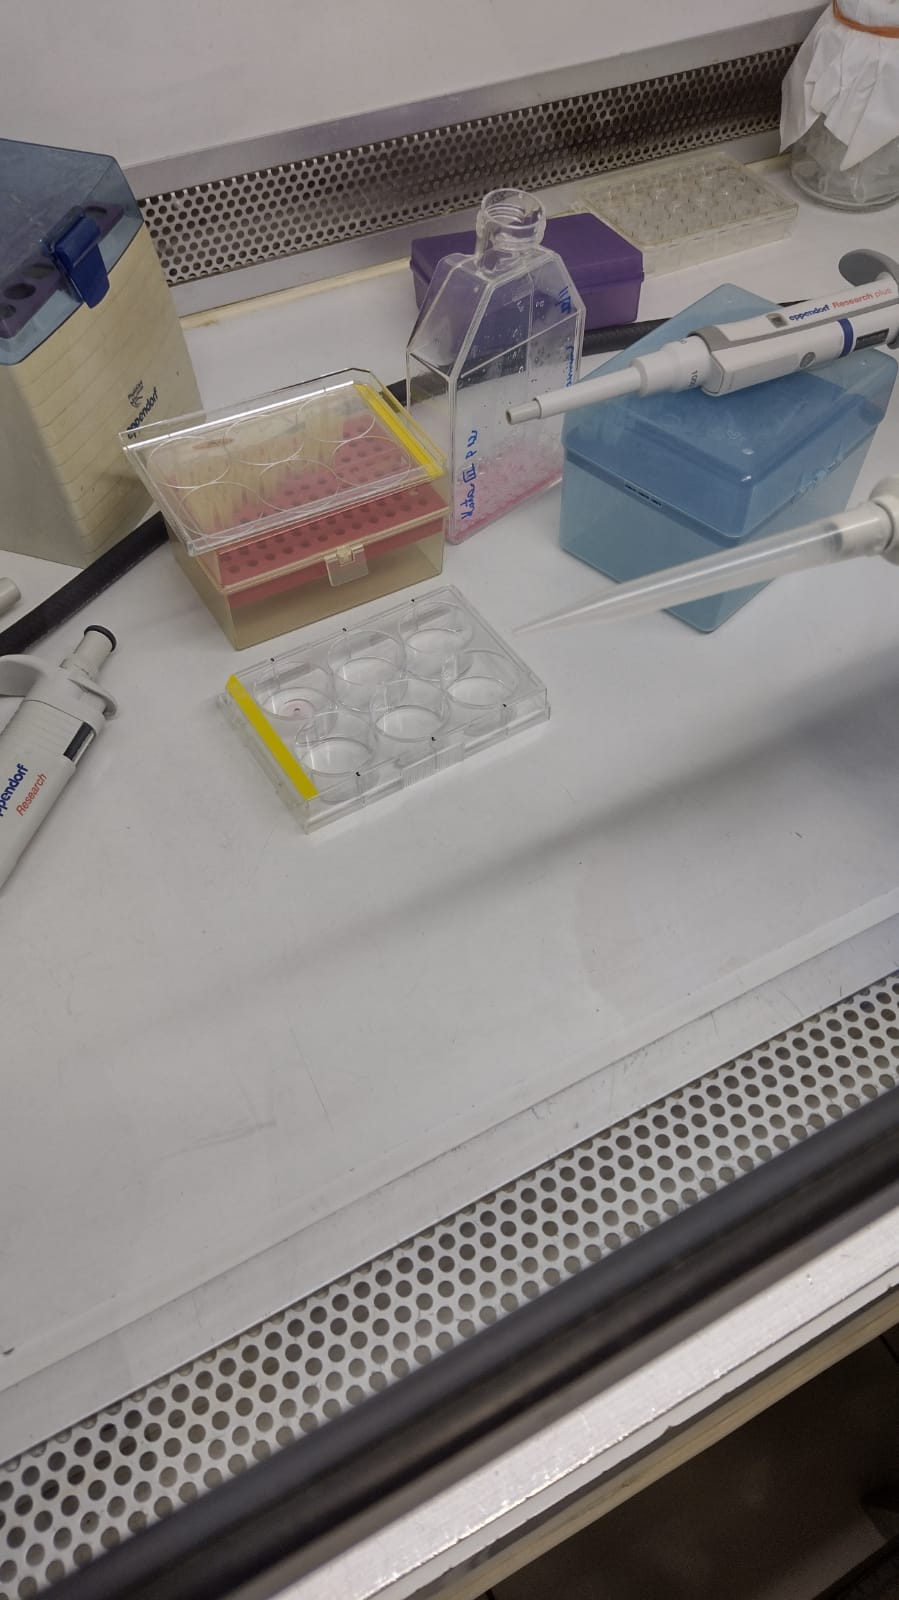
\includegraphics[width=2cm]{figures/datasets/spheroid_2}} \\
        \subfloat{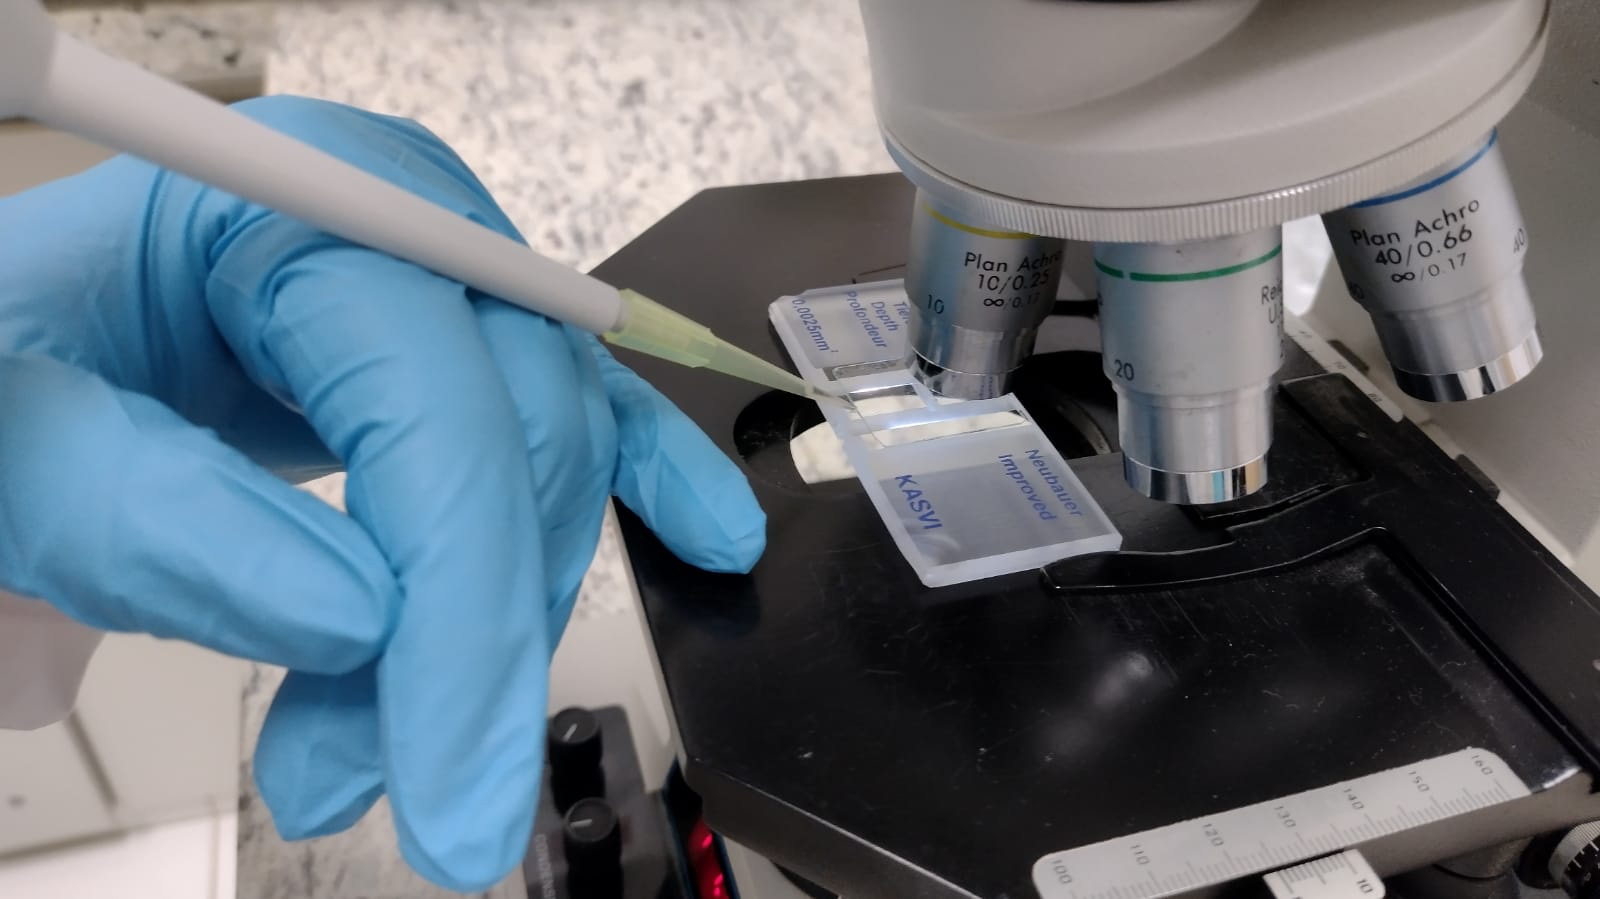
\includegraphics[width=4cm]{figures/datasets/spheroid_3}}
        \subfloat{
\includegraphics[width=4cm]{figures/datasets/spheroid_4}}
    \end{figure}
\end{frame}

%---------------------------------------------------------
\begin{frame}{Image Acquisition}
    \begin{figure}[!htb]
        \centering
        \subfloat[$48$h]{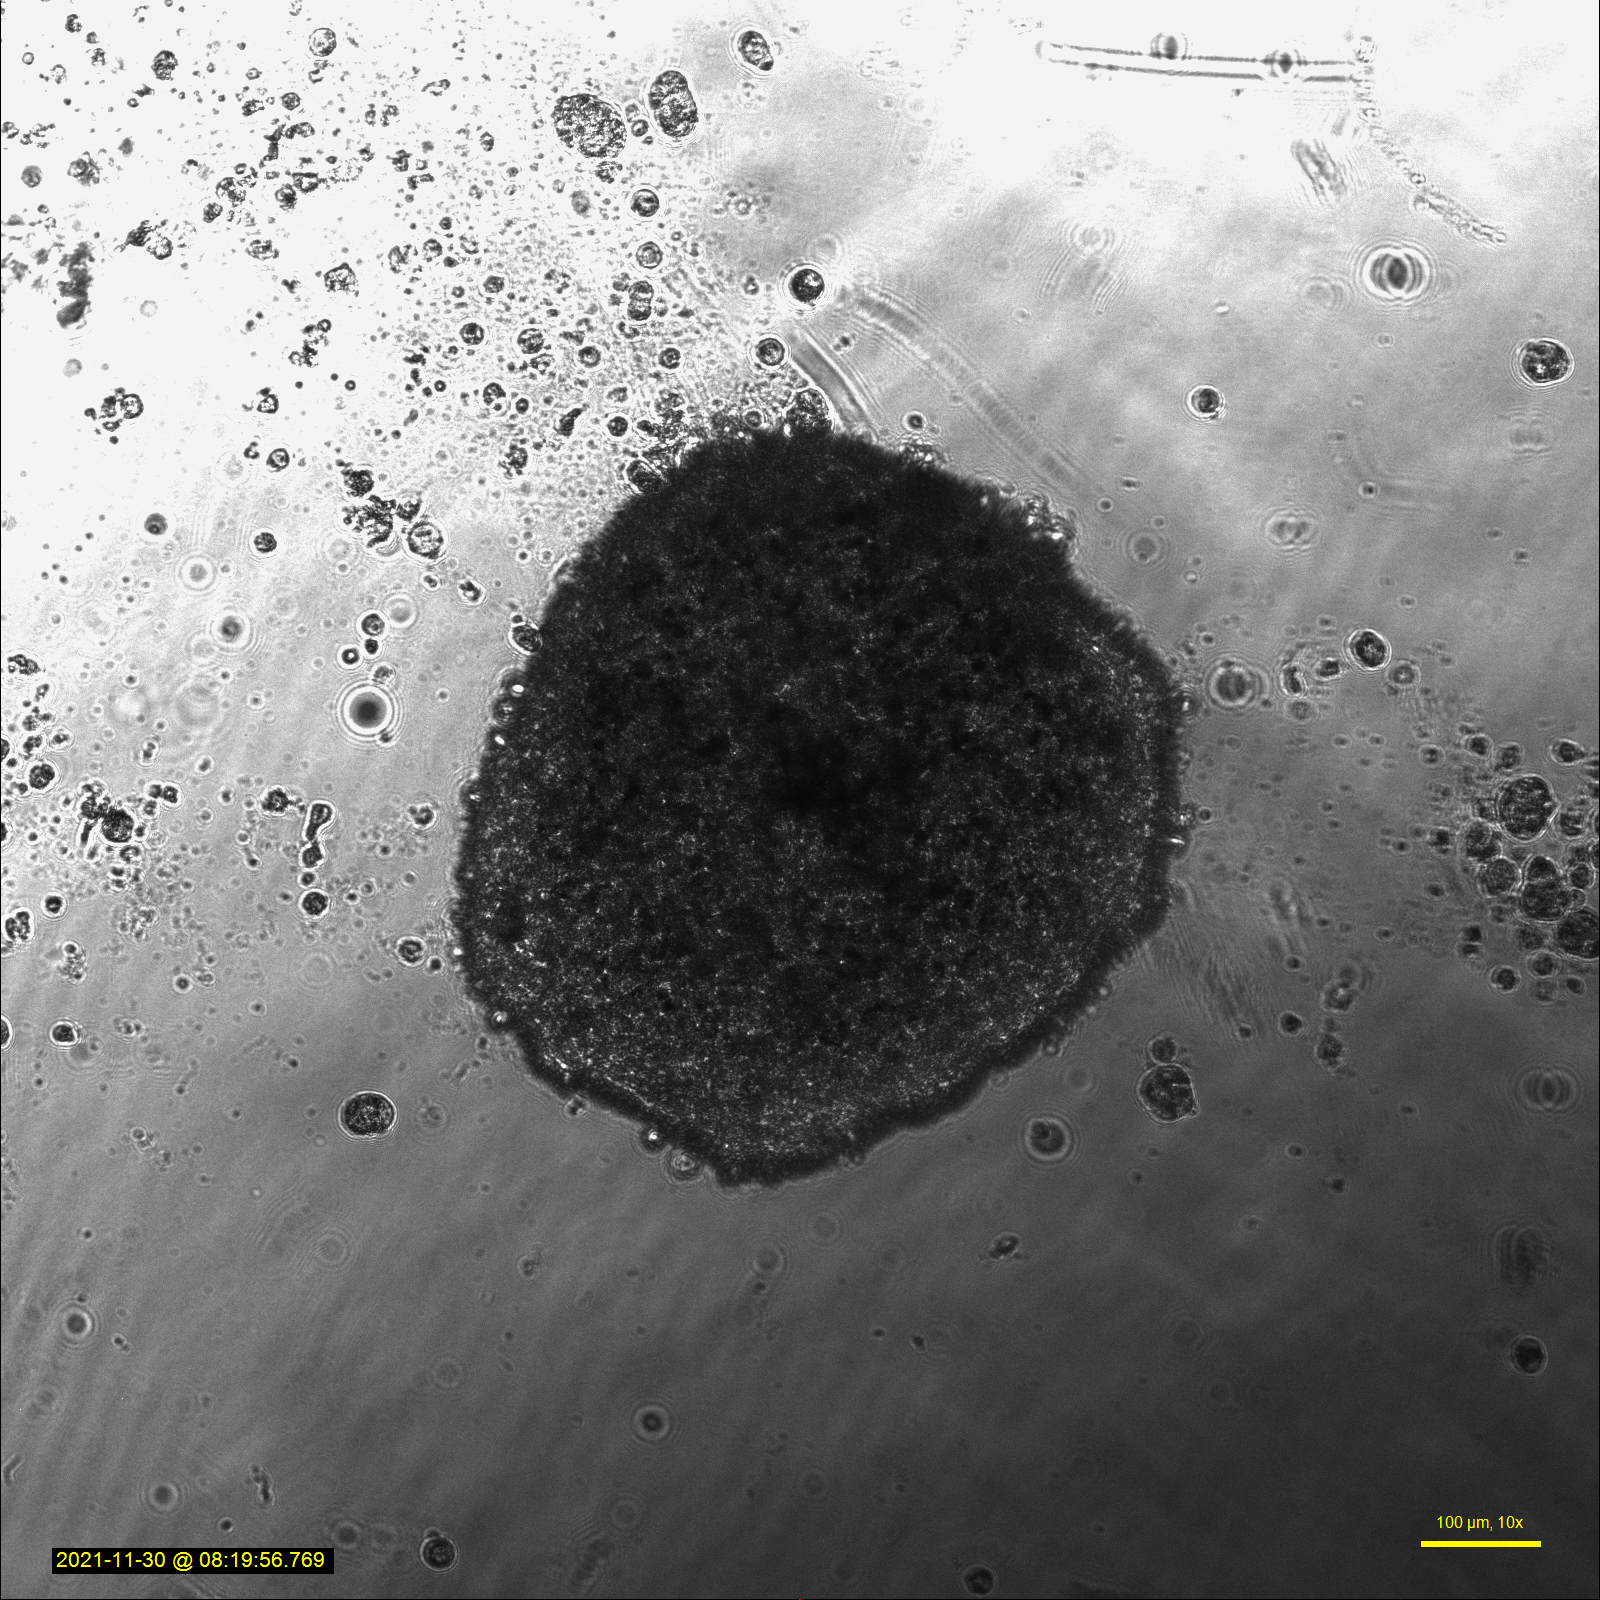
\includegraphics[width=4cm]{figures/datasets/48_B12N}}
        \subfloat[$72$h]{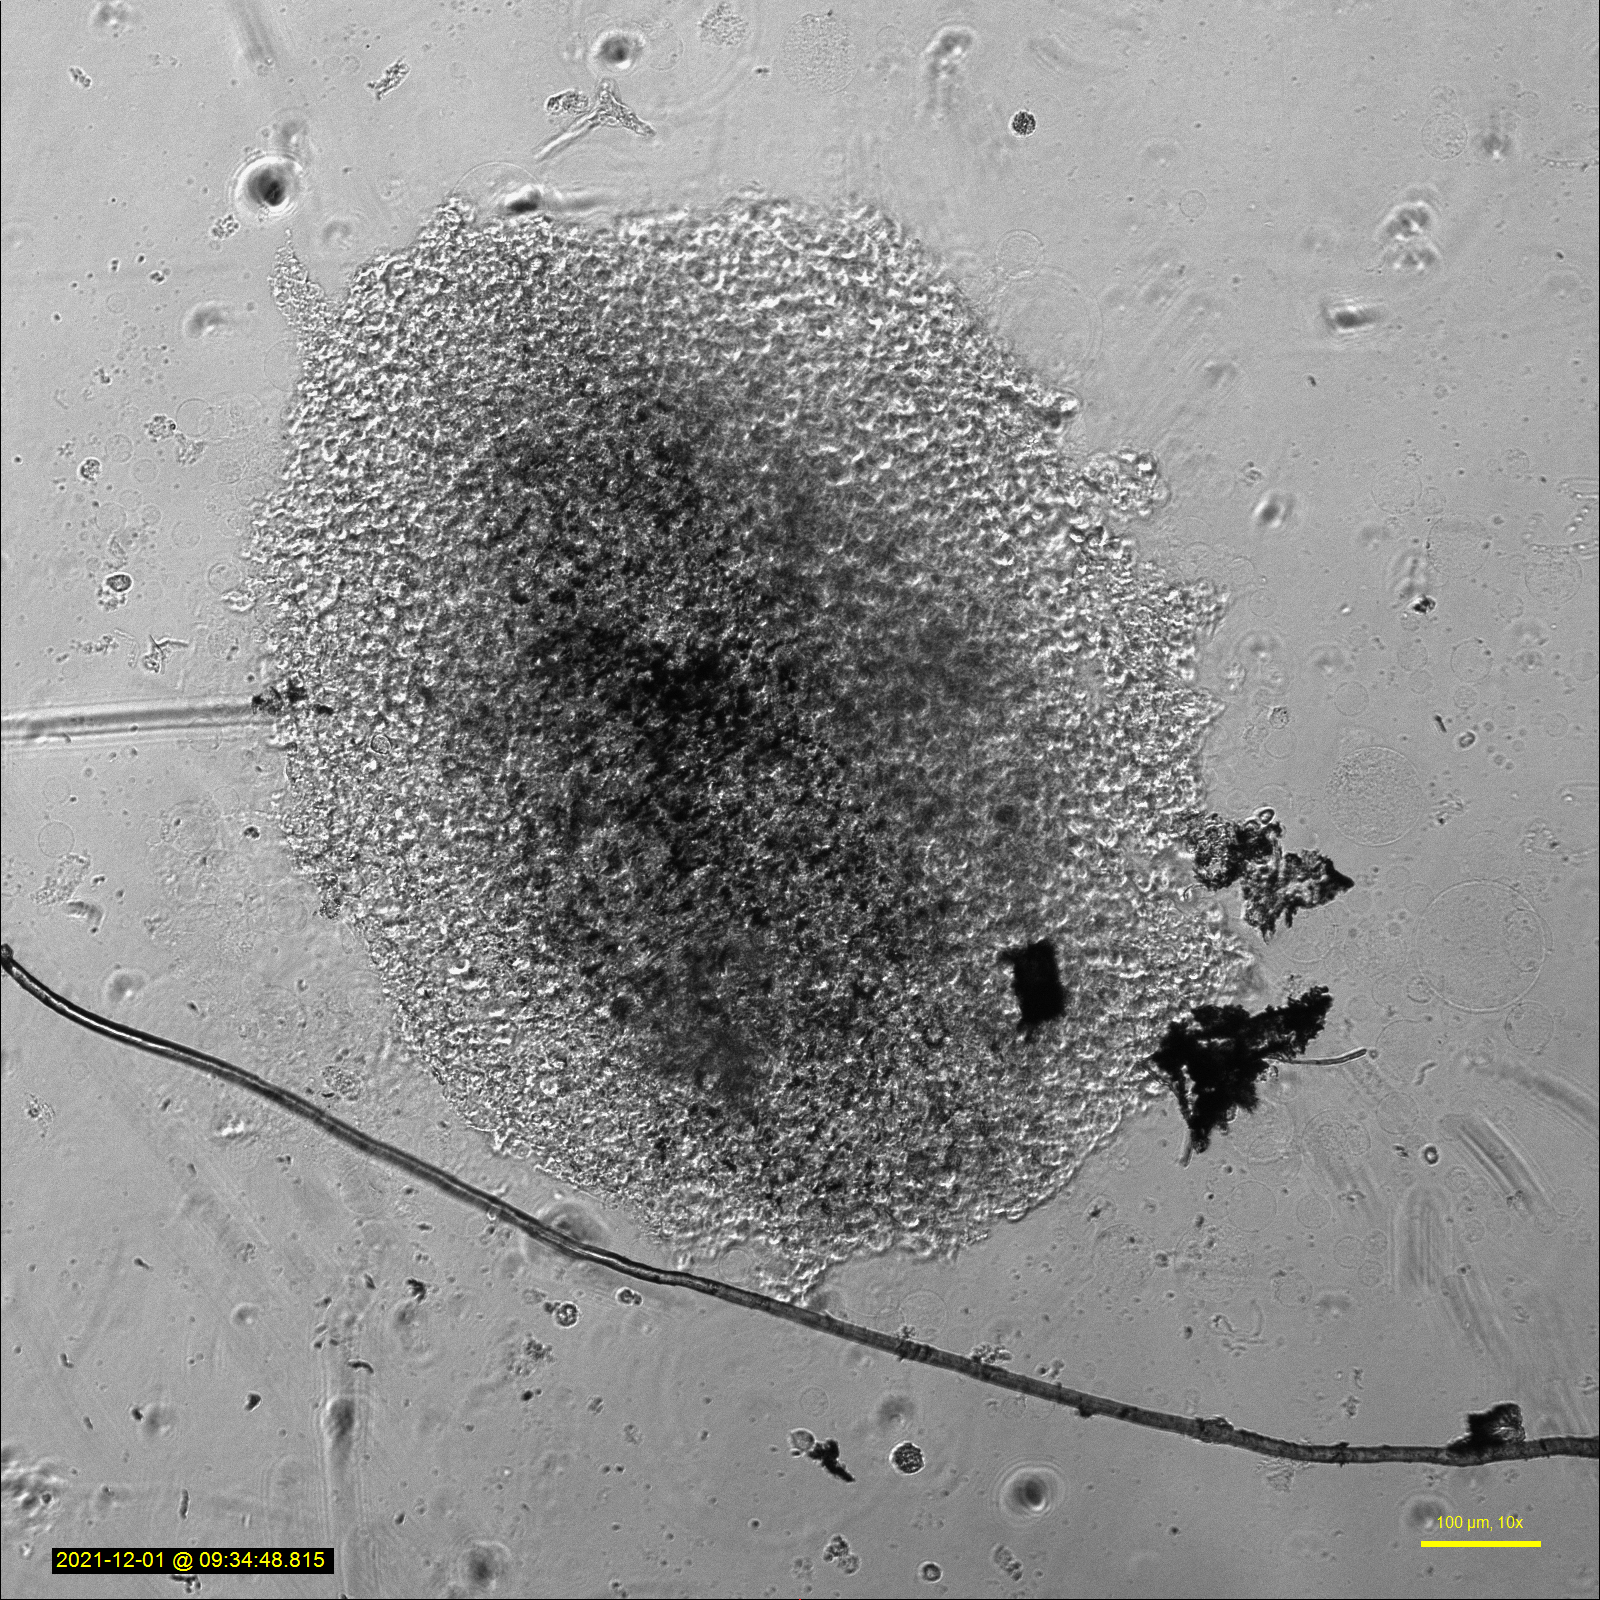
\includegraphics[width=4cm]{figures/datasets/72_B12N}}
        \subfloat[$96$h]{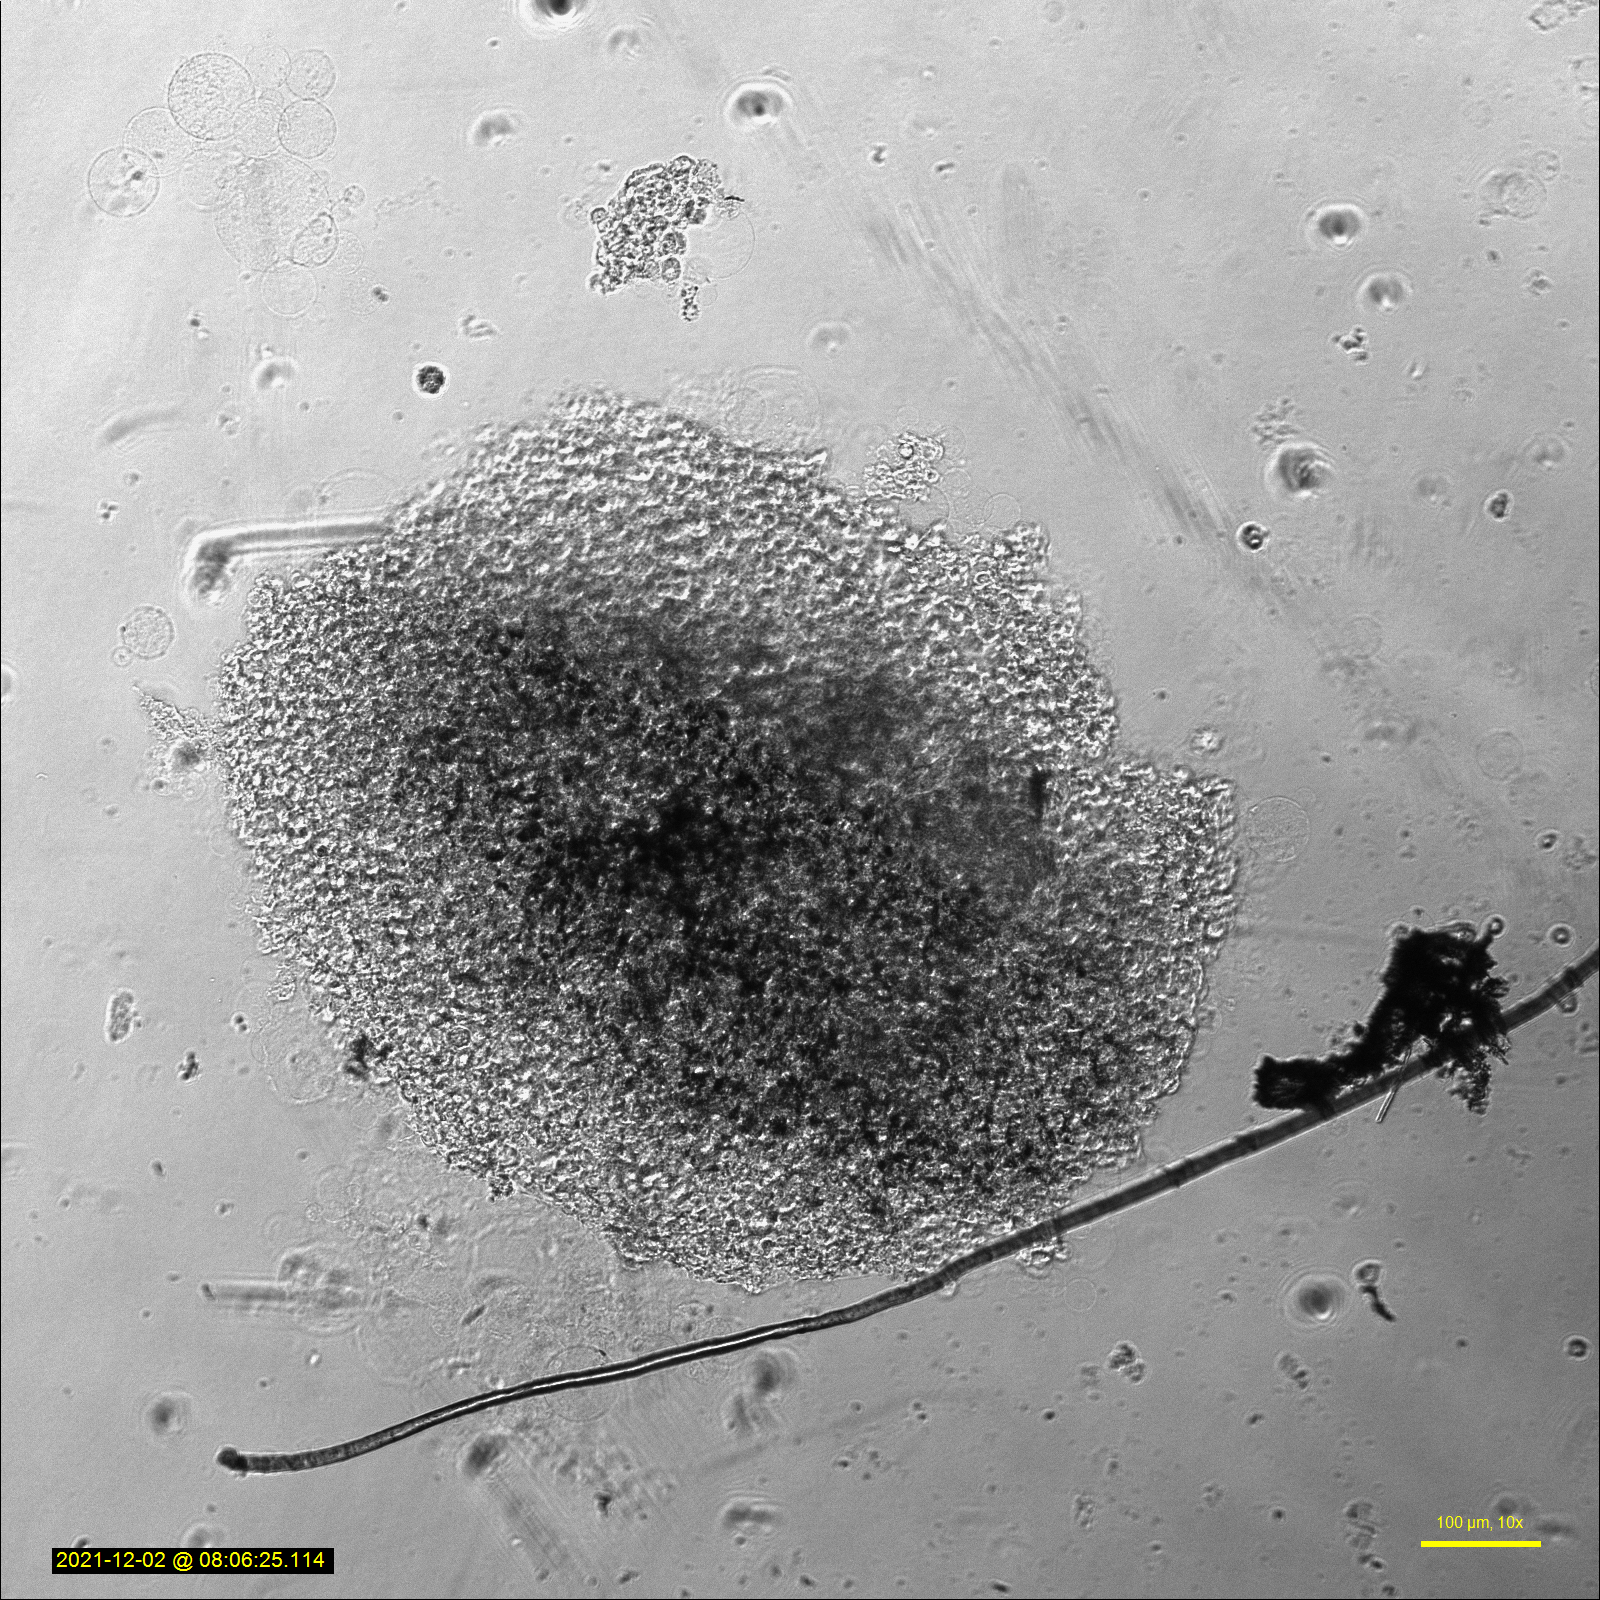
\includegraphics[width=4cm]{figures/datasets/96_B12N}}
    \end{figure}
\end{frame}
\setBGColor{UFGBlue}
\section{Method}

\setLayout{mainpoint}

\begin{frame}[noframenumbering, plain]{}
    \frametitle{Method}
\end{frame}

\setLayout{blank}

%---------------------------------------------------------
\begin{frame}{Overview}
    \begin{figure}[!htb]
    \centering
        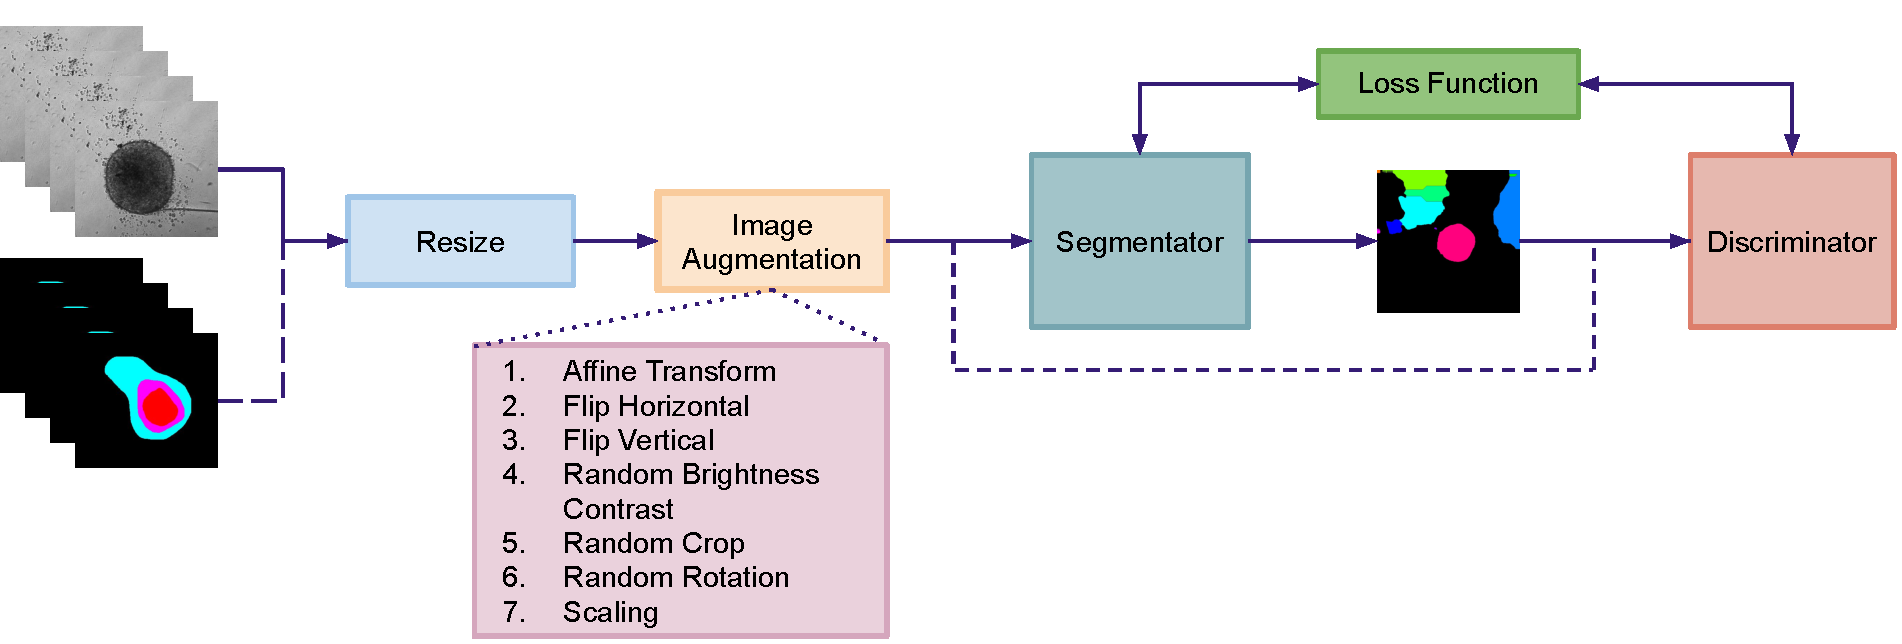
\includegraphics[width=15cm]{figures/method/overview}
        \label{fig:method_overview}
    \end{figure}
\end{frame}

%---------------------------------------------------------
\setLayout{horizontal}

\begin{frame}{Data Augmentation}
    \begin{figure}
        \centering
        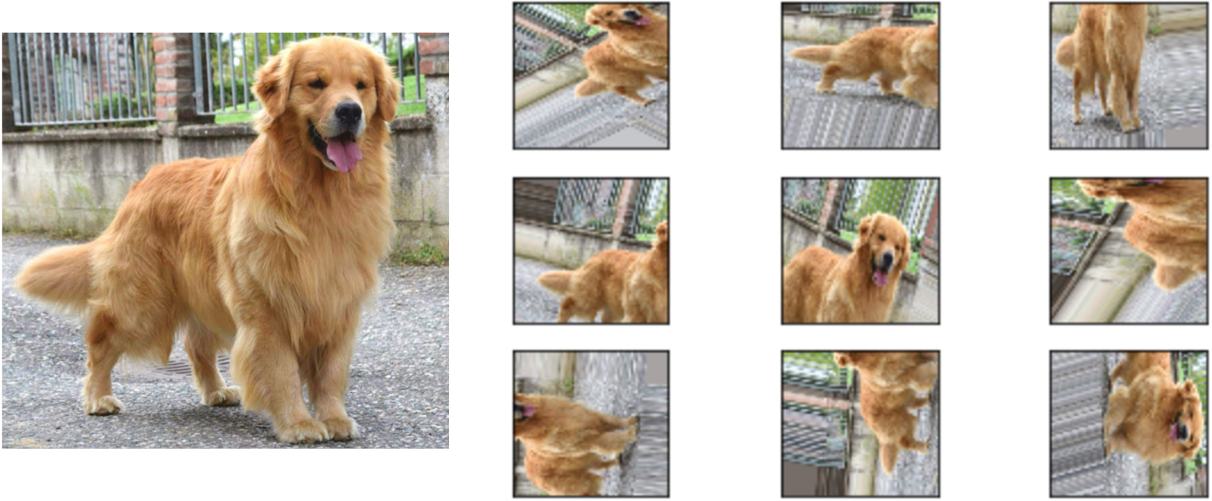
\includegraphics[width=13cm]{figures/method/data_augmentation}
    \end{figure}
\end{frame}

%---------------------------------------------------------
\setLayout{blank}

\begin{frame}{Generator Architecture}
    \begin{figure}[!htb]
        \centering
        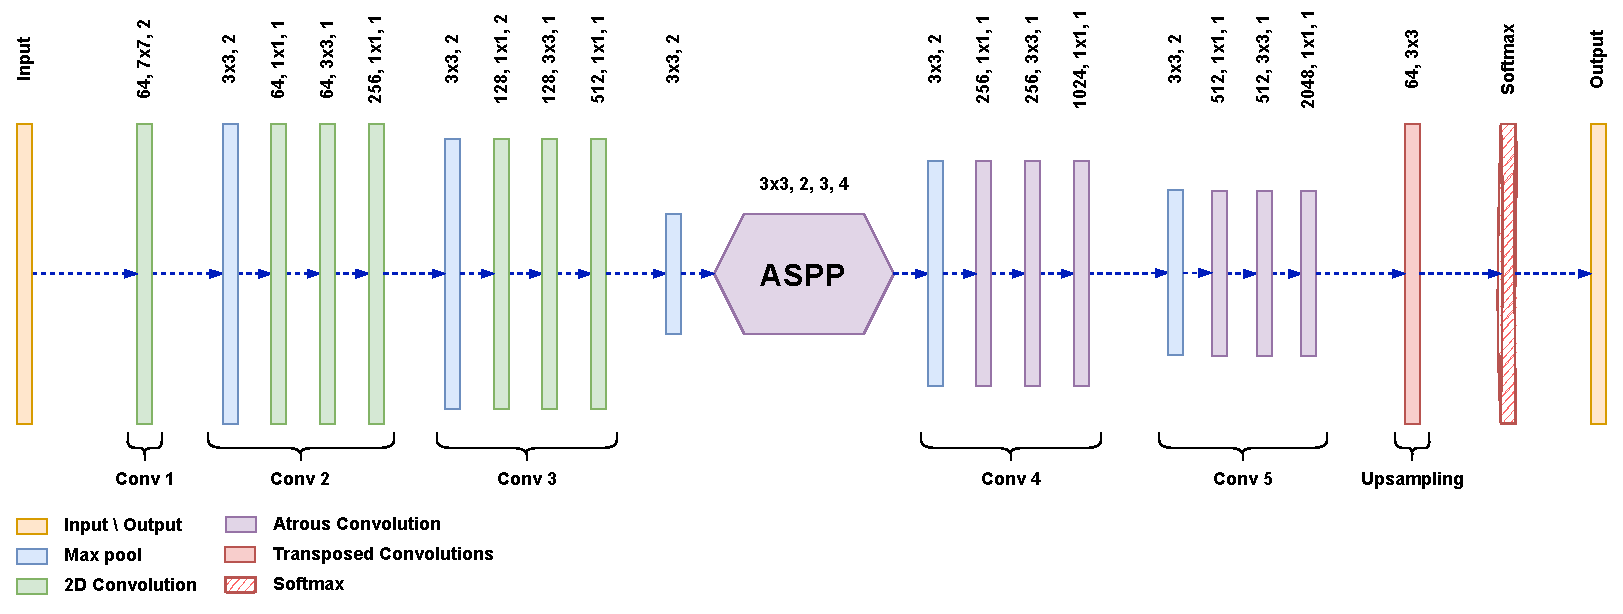
\includegraphics[width=14cm]{figures/method/generator_architecture}
    \end{figure}
\end{frame}

%---------------------------------------------------------

\begin{frame}{Discriminator Architecture}
    \begin{figure}[!htb]
        \centering
        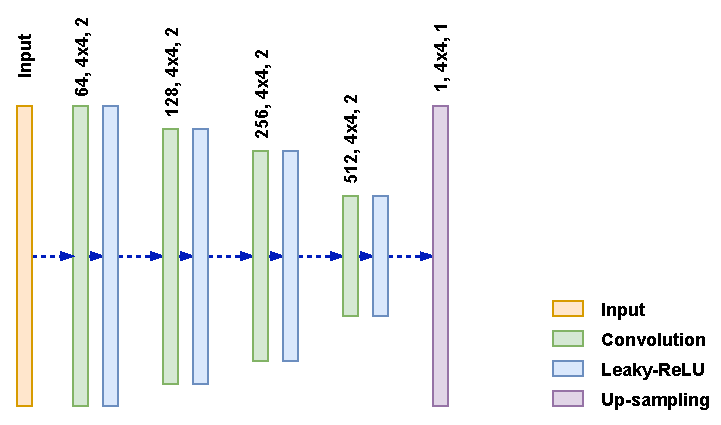
\includegraphics[width=10cm]{figures/method/discriminator_architecture}
    \end{figure}
\end{frame}

%---------------------------------------------------------
\setLayout{vertical}

\begin{frame}{Loss Functions}
    \begin{block}{Generator Loss}
        \begin{equation}
            \label{eq:seg_loss}
            \mathcal{L}_{seg} = \mathcal{L}_{ce} + \lambda_{adv}\mathcal{L}_{adv} + \lambda_{semi}\mathcal{L}_{semi}
        \end{equation}
    \end{block}
\end{frame}

%---------------------------------------------------------
\begin{frame}{Evaluation Metrics}
    \begin{columns}
        \column{0.5\textwidth}
        Dice Coefficient
        \begin{figure}[!htb]
            \centering
            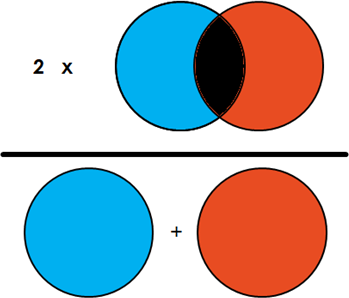
\includegraphics[width=5cm]{figures/method/dice_coefficient}
        \end{figure}
        \column{0.5\textwidth}
        Jaccard Index
        \begin{figure}[!htb]
            \centering
            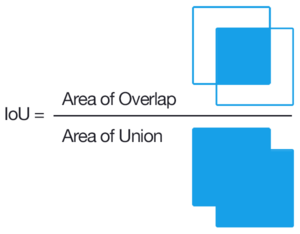
\includegraphics[width=5cm]{figures/method/jaccard_index}
        \end{figure}
    \end{columns}
\end{frame}

%---------------------------------------------------------
\setLayout{horizontal}

\begin{frame}{Watershed}
    \begin{figure}
        \centering
        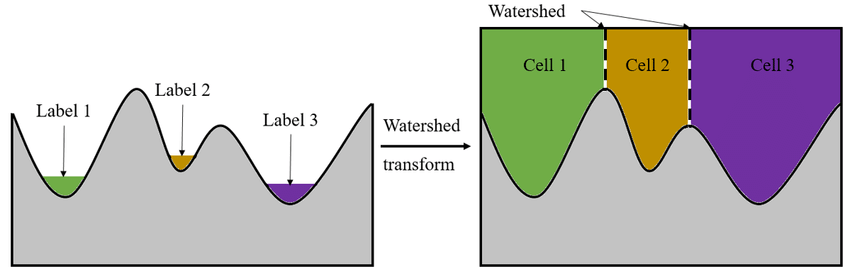
\includegraphics[width=15cm]{figures/method/watershed}
    \end{figure}
\end{frame}

\setBGColor{LightOrange}
\section{Preliminary Results}

\setLayout{mainpoint}

\begin{frame}[noframenumbering, plain]{}
    \frametitle{Preliminary Results}
\end{frame}

\setLayout{horizontal}

%---------------------------------------------------------
\begin{frame}{Comparative Table}
    Metric used: \alert{Mean Jaccard}.
    \begin{table}[]
        \centering
        \setlength{\tabcolsep}{10pt}
        
        {\rowcolors{2}{}{LightGray!10}
            \begin{tabular}{lccccccc}
                Method & BL5S & BN10S & BN2S & FL5C & FL5S & FN2S & Ours \\
                \midrule
                Watershed & $0.73$ & $0.64$ & $0.45$ &  $0.63$ & $0.44$ & $0.41$ & - \\
                U-Net & $0.75^*$ & - & - & $0.93$ & - & - & -
            \end{tabular}
        }
    \end{table}
\end{frame}

%---------------------------------------------------------
\setLayout{blank}

%---------------------------------------------------------
\begin{frame}{BL5S - 0.73}
    \begin{figure}[!htb]
        \centering
        \subfloat{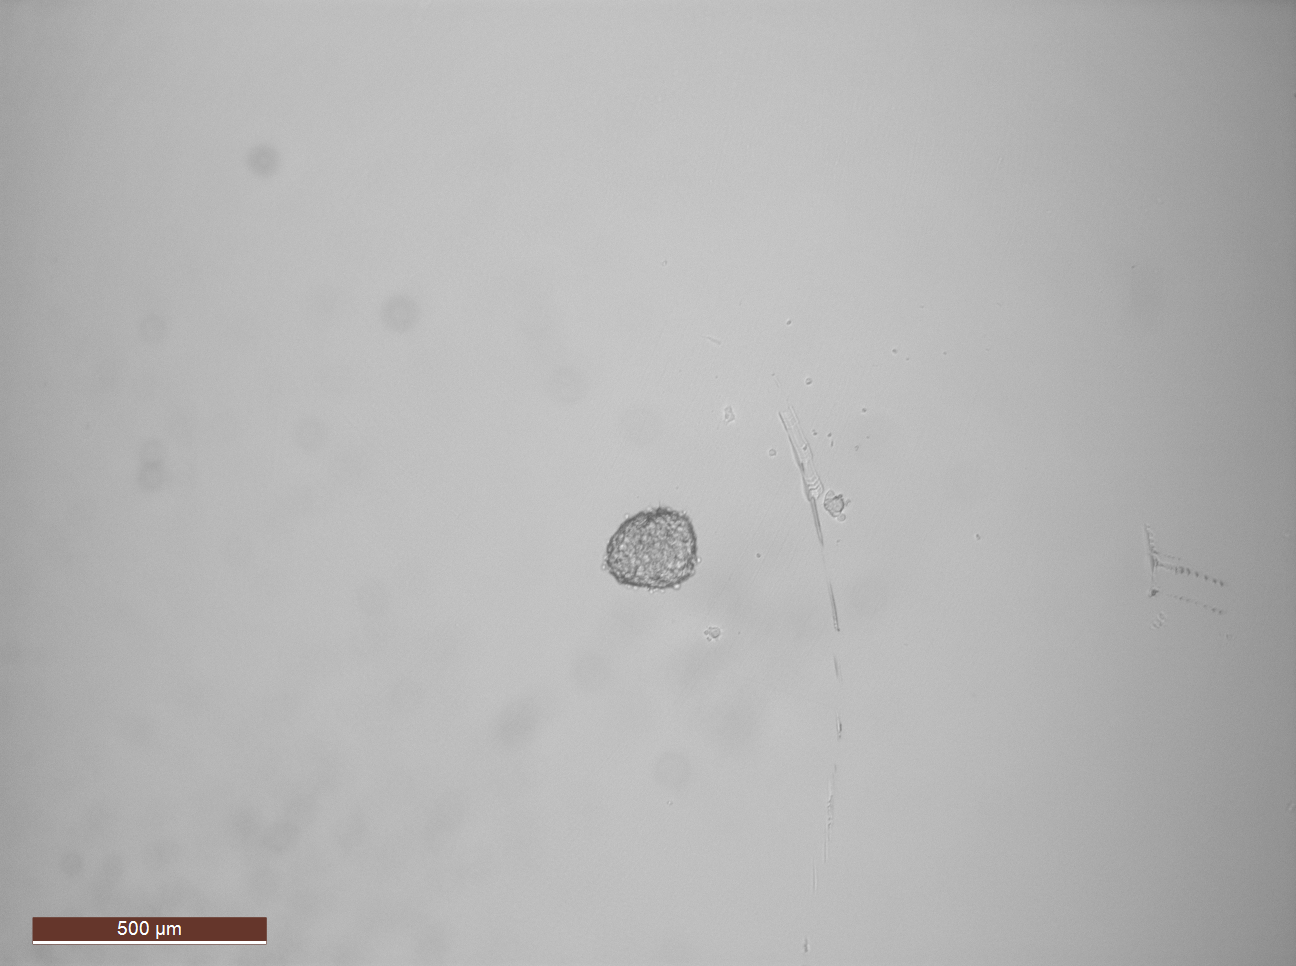
\includegraphics[width=3cm]{figures/result/bl5s_02_image}}
        \subfloat{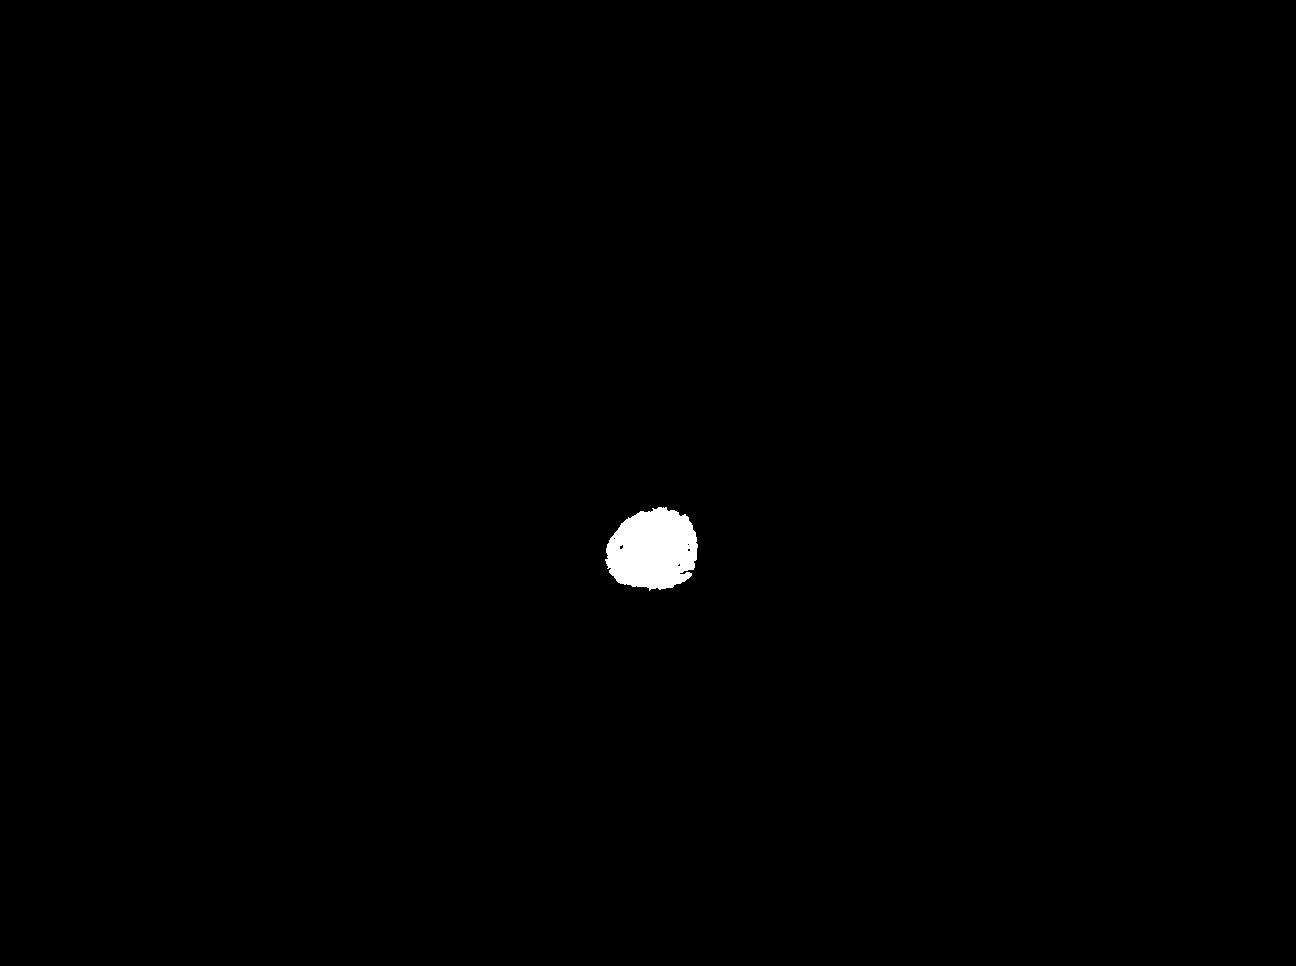
\includegraphics[width=3cm]{figures/result/bl5s_02_pred}}
        \subfloat{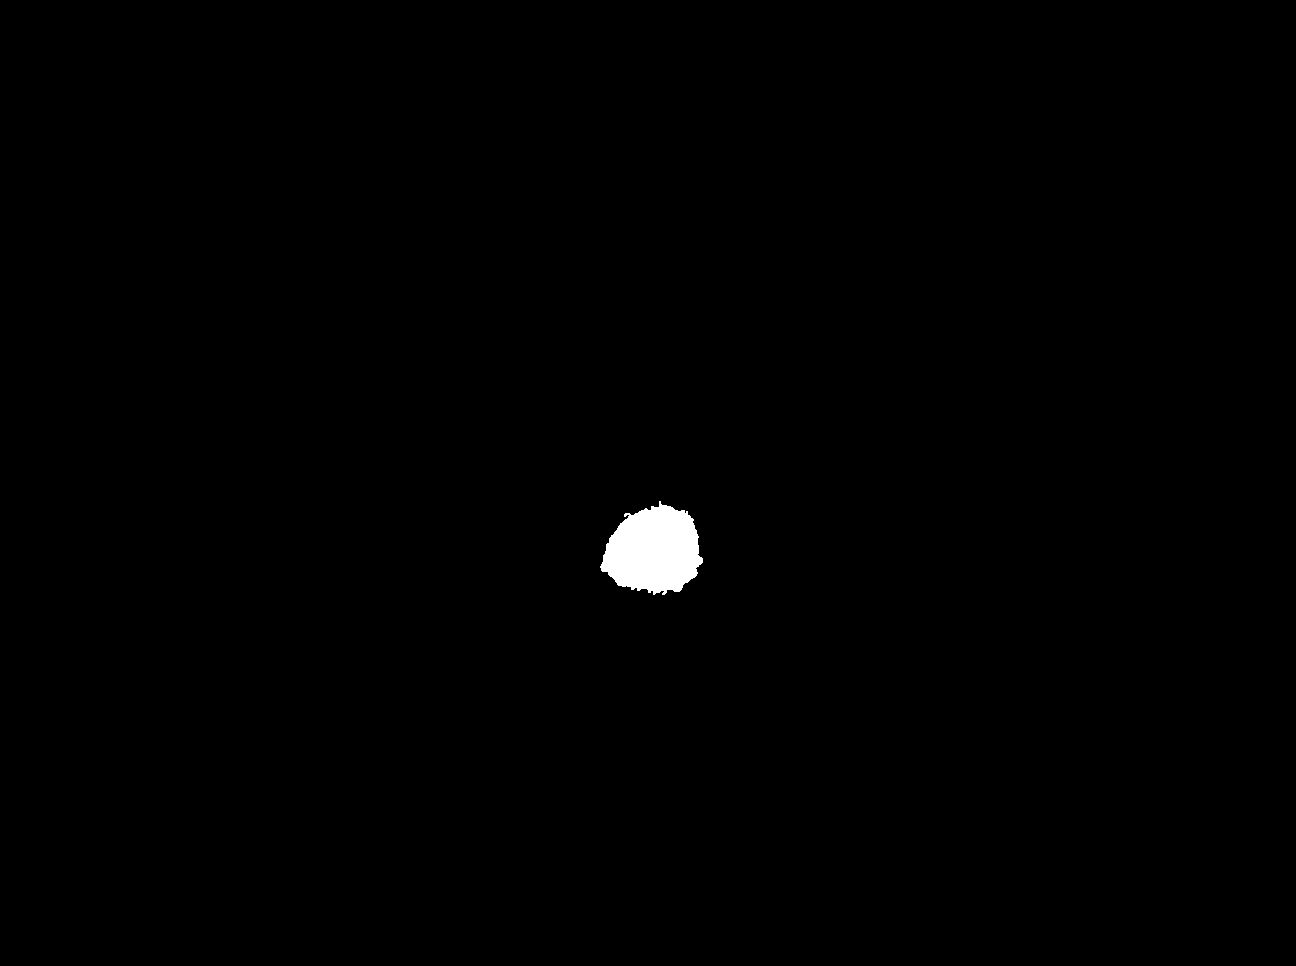
\includegraphics[width=3cm]{figures/result/bl5s_02_gt}}\\
        \subfloat{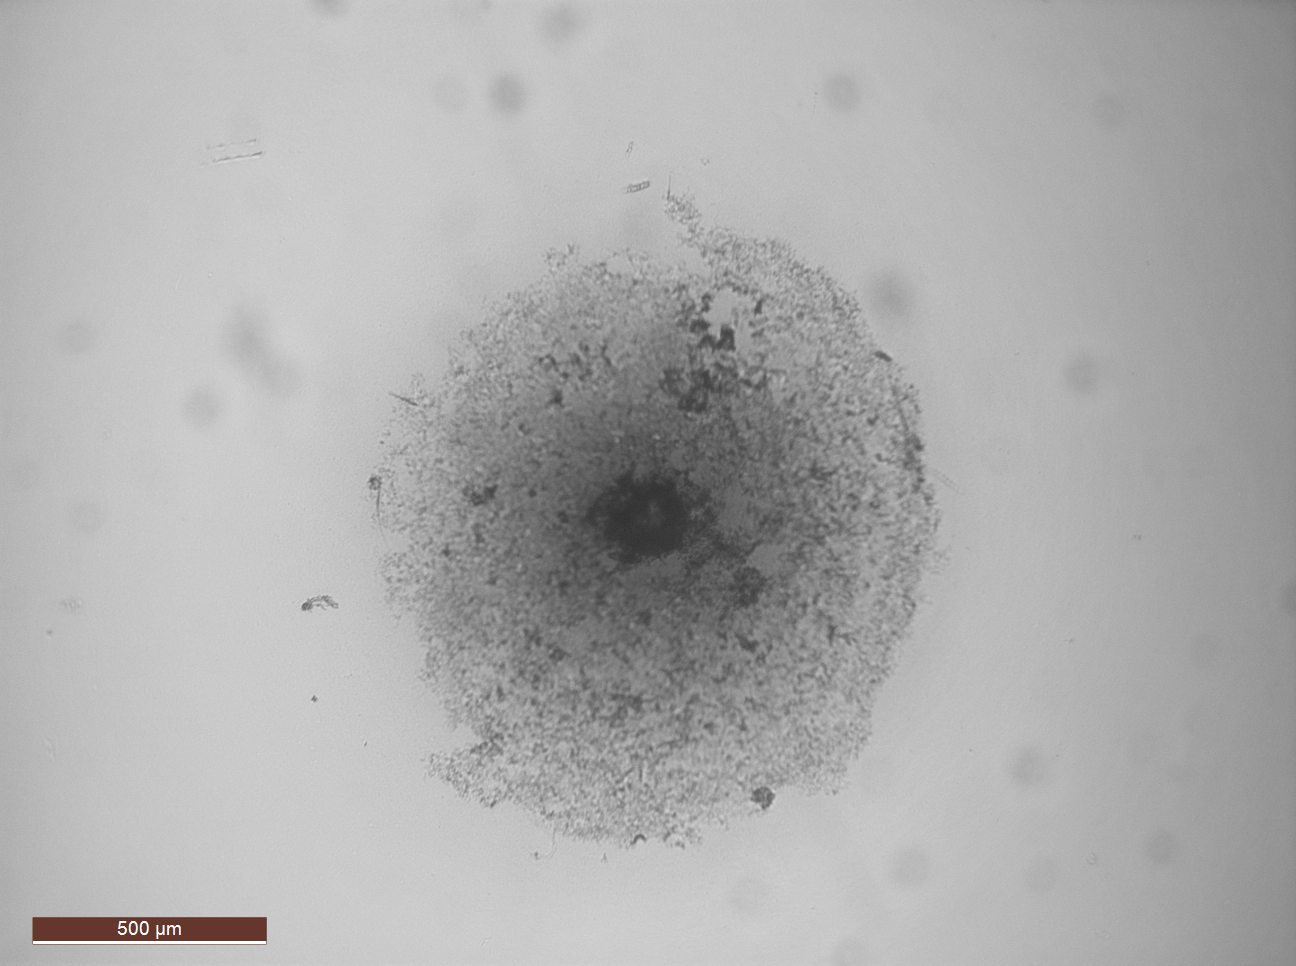
\includegraphics[width=3cm]{figures/result/bl5s_28_image}}
        \subfloat{
\includegraphics[width=3cm]{figures/result/bl5s_28_pred}}
        \subfloat{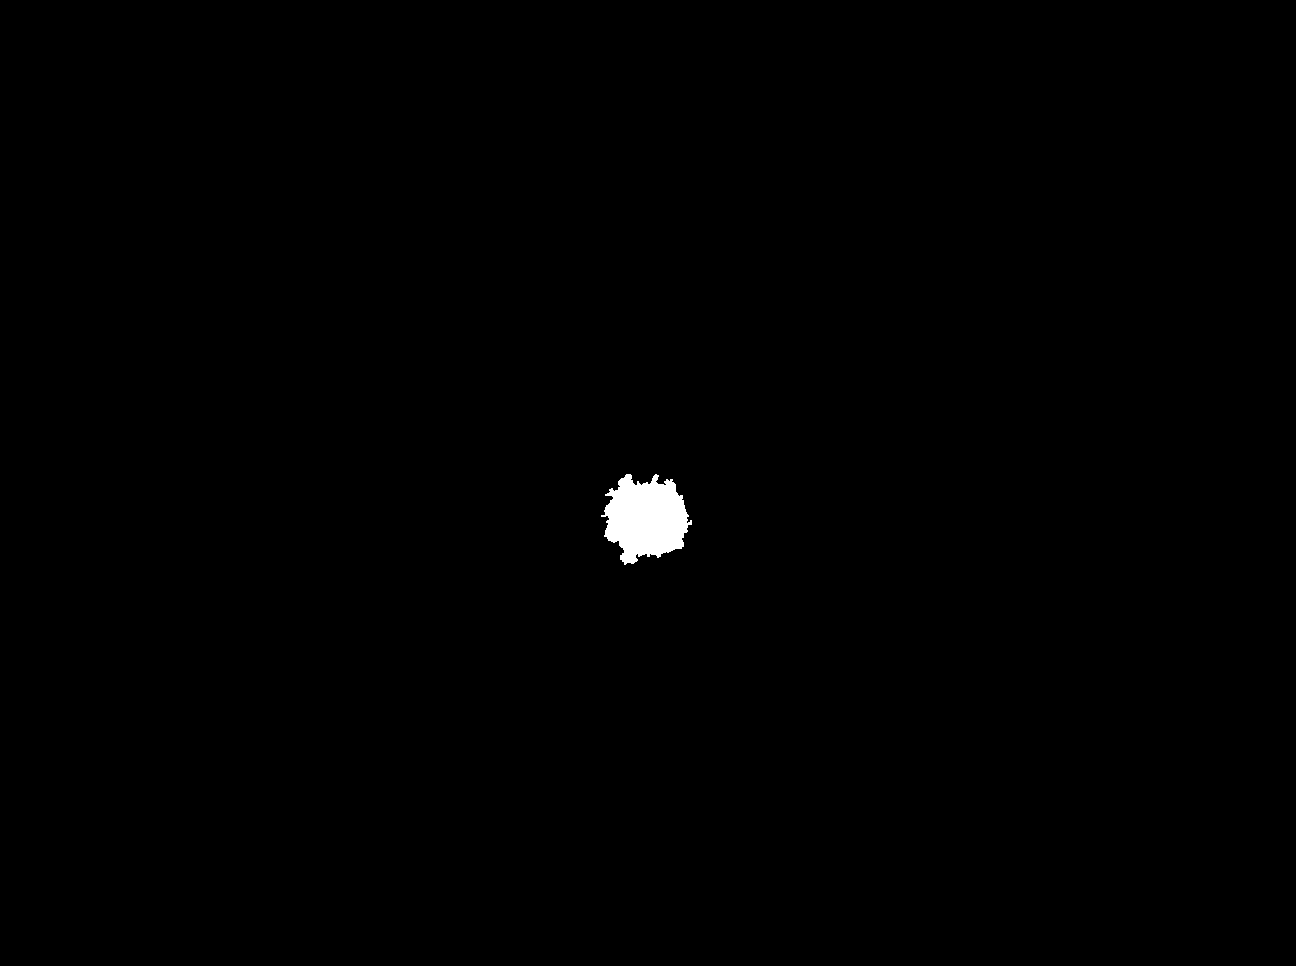
\includegraphics[width=3cm]{figures/result/bl5s_28_gt}}\\
        \subfloat{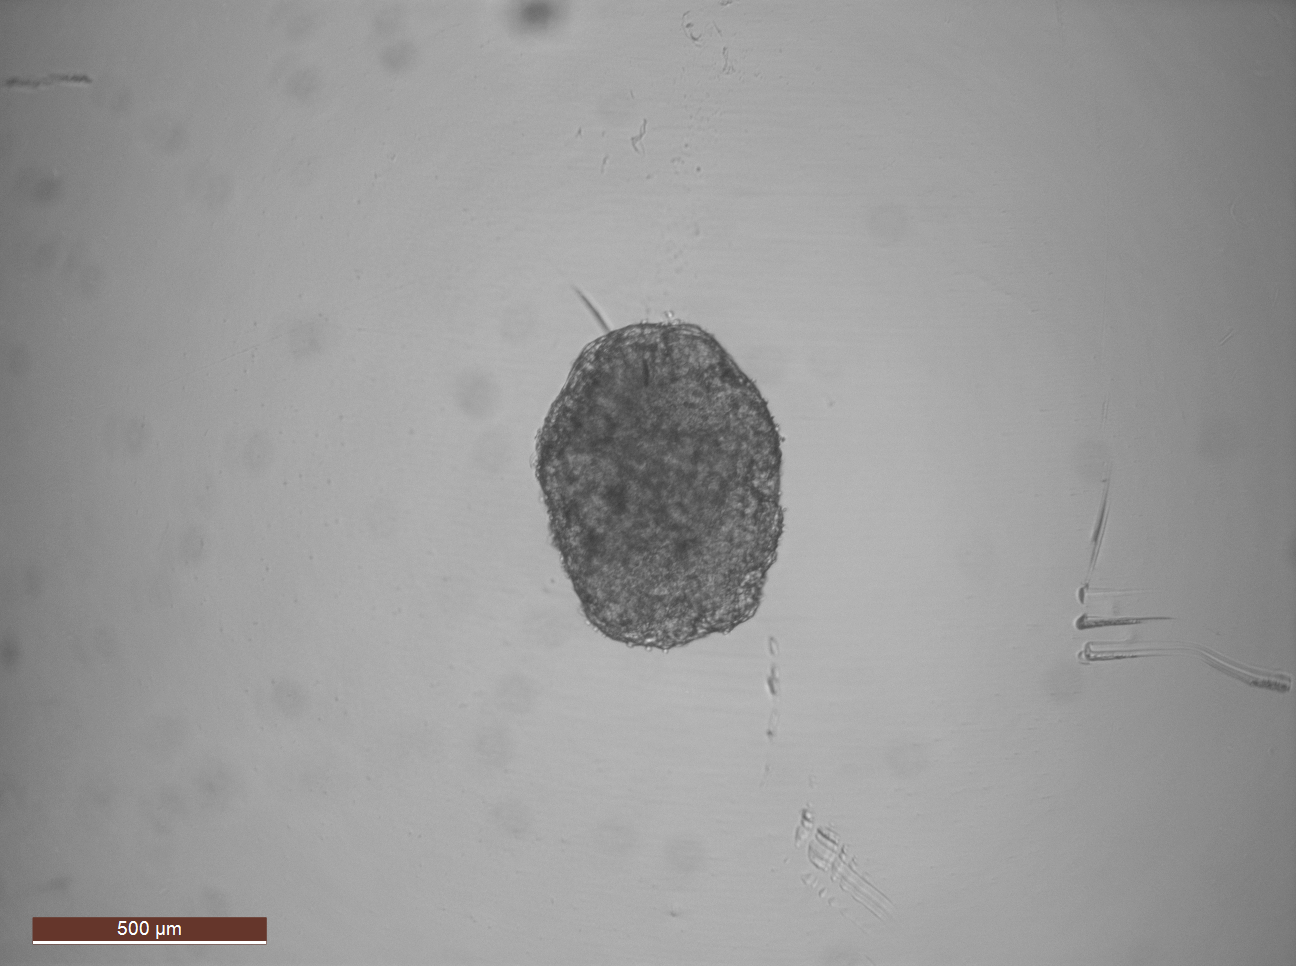
\includegraphics[width=3cm]{figures/result/bl5s_31_image}}
        \subfloat{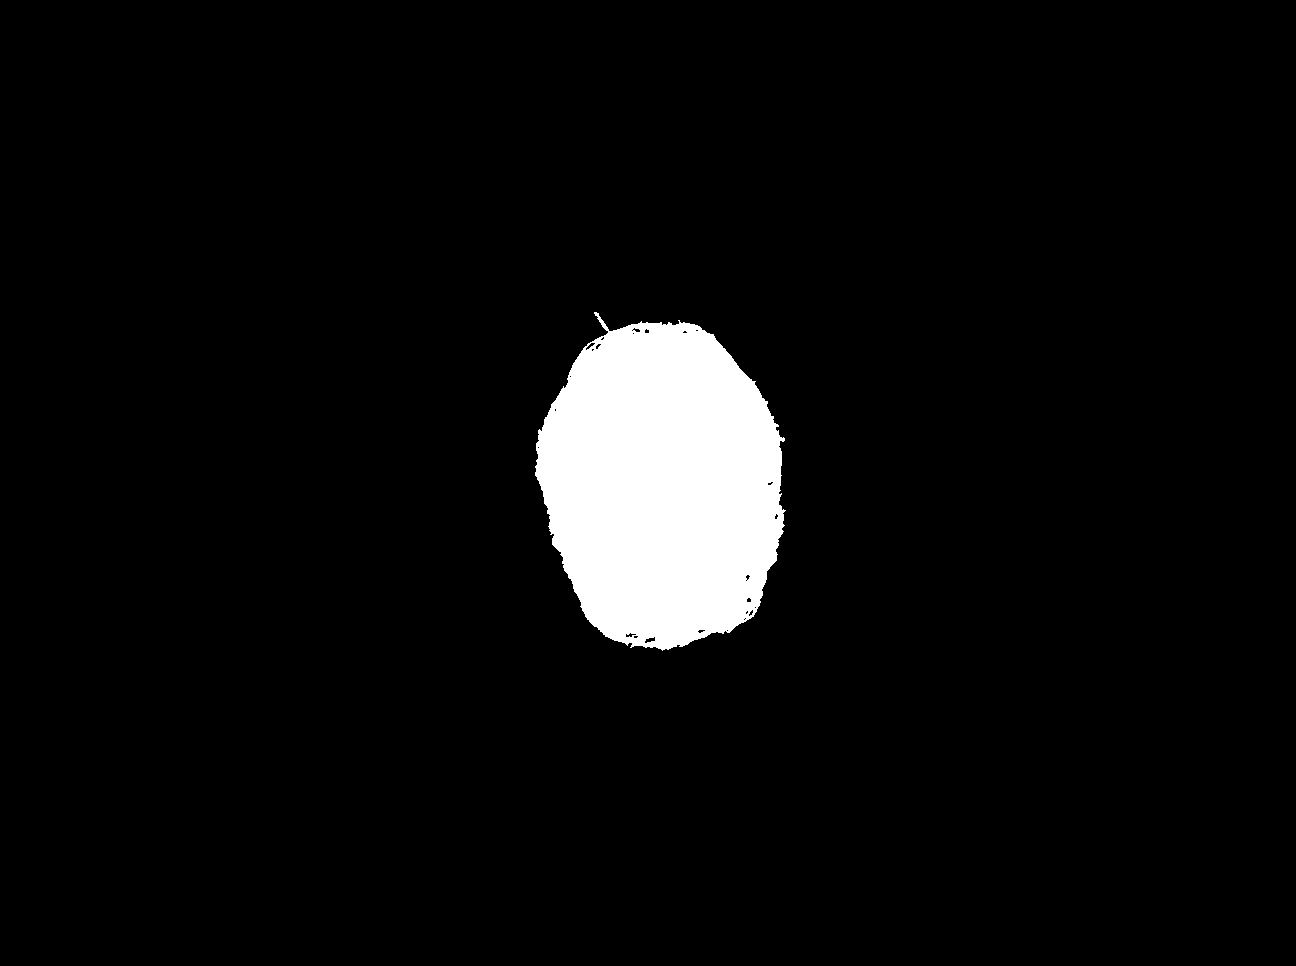
\includegraphics[width=3cm]{figures/result/bl5s_31_pred}}
        \subfloat{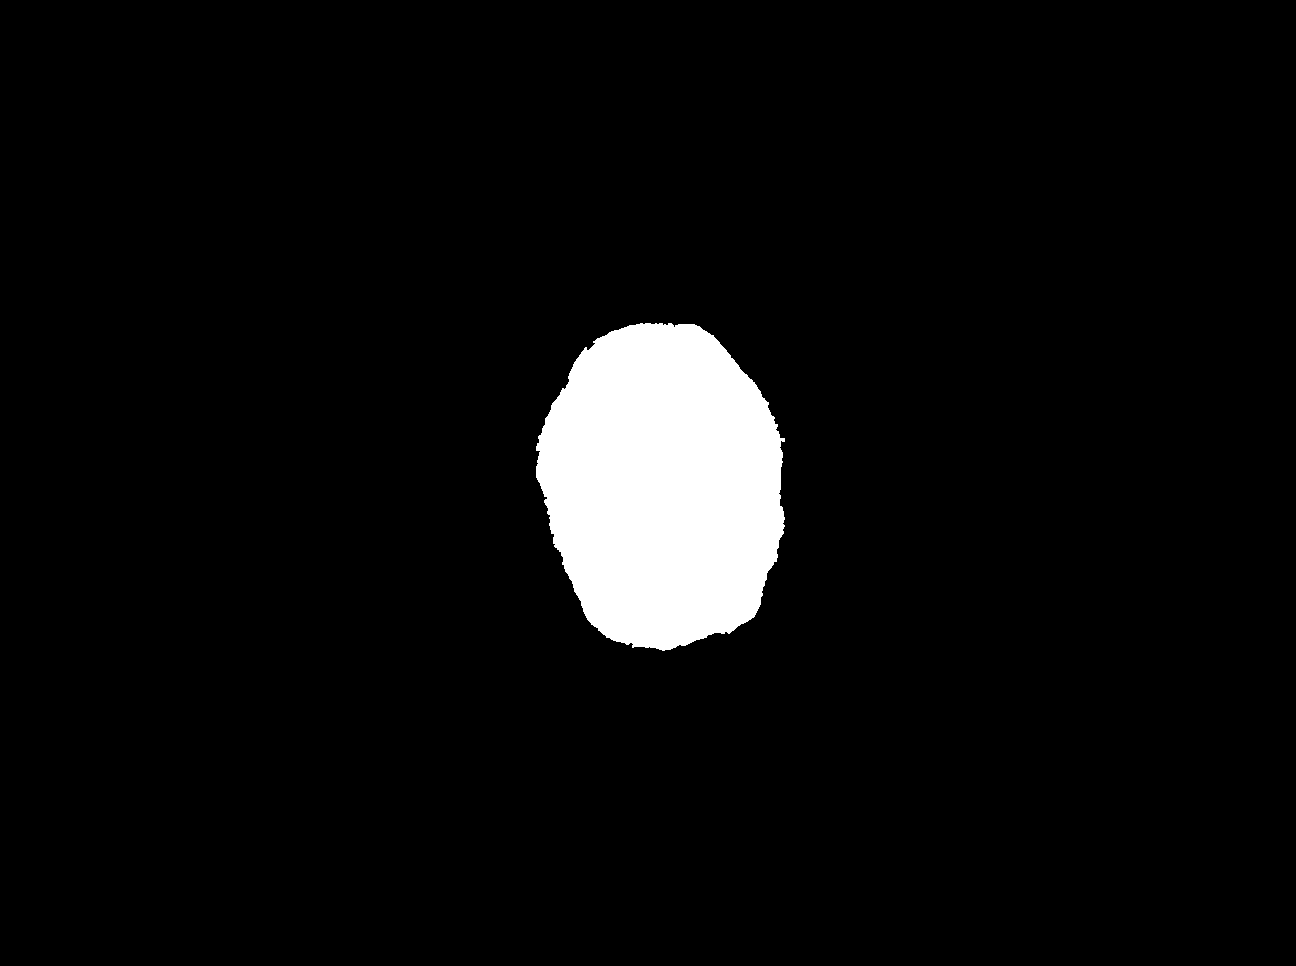
\includegraphics[width=3cm]{figures/result/bl5s_31_gt}}
    \end{figure}
\end{frame}

%---------------------------------------------------------
\begin{frame}{BN10S - 0.64}
    \begin{figure}[!htb]
        \centering
        \subfloat{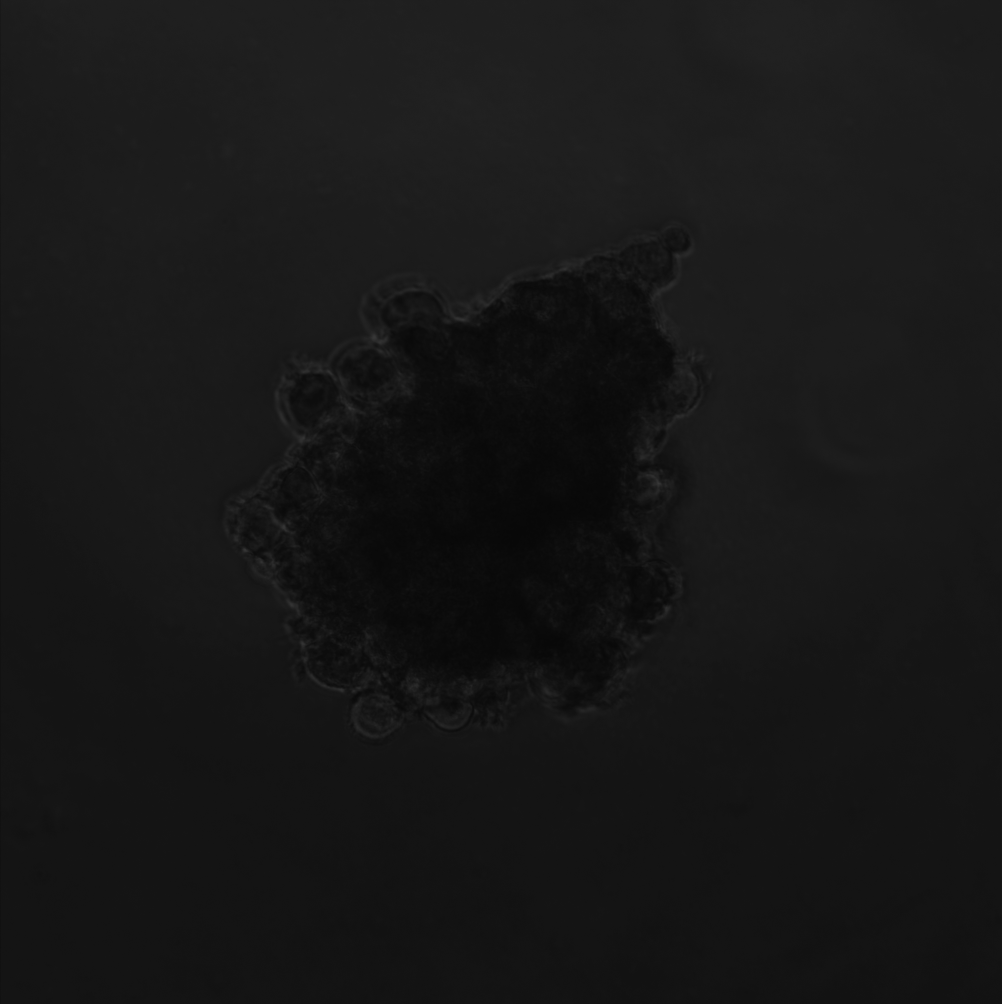
\includegraphics[width=2cm]{figures/result/bn10s_61_image}}
        \subfloat{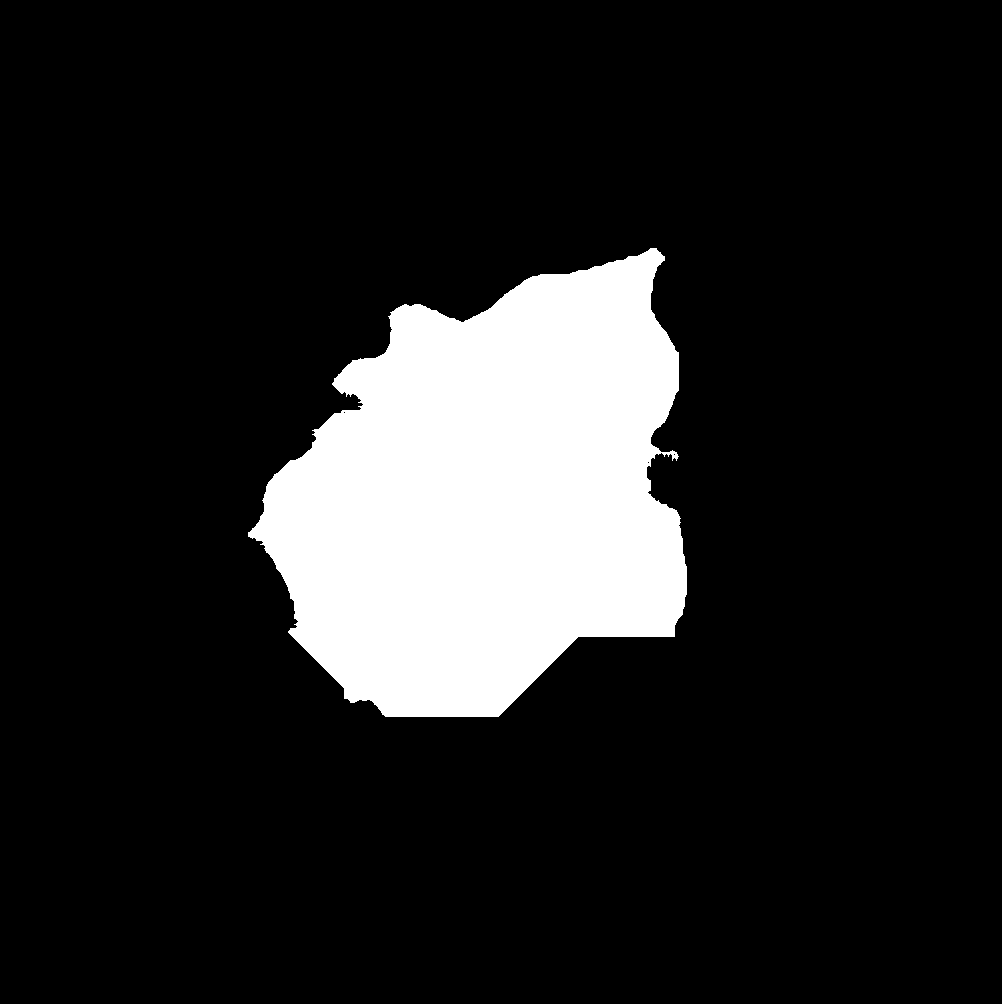
\includegraphics[width=2cm]{figures/result/bn10s_61_pred}}
        \subfloat{
\includegraphics[width=2cm]{figures/result/bn10s_61_gt}}\\
        \subfloat{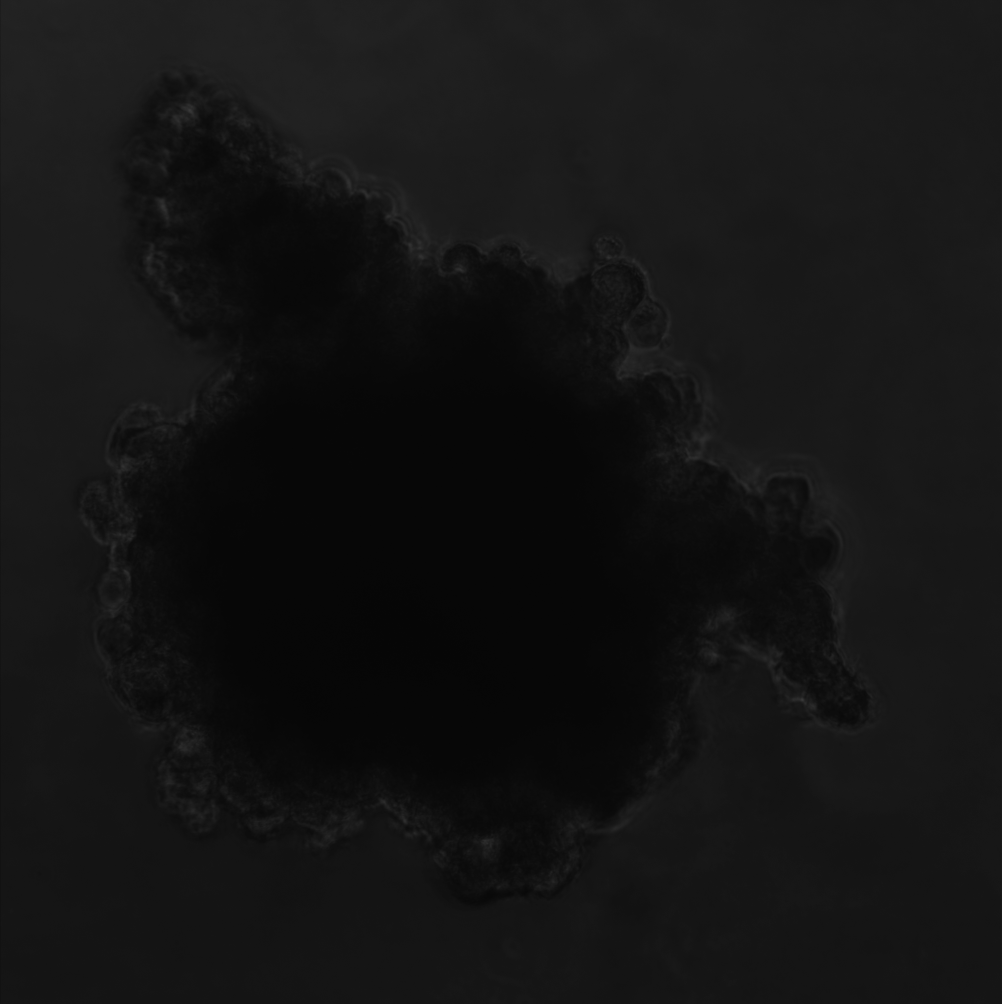
\includegraphics[width=2cm]{figures/result/bn10s_45_image}}
        \subfloat{
\includegraphics[width=2cm]{figures/result/bn10s_45_pred}}
        \subfloat{
\includegraphics[width=2cm]{figures/result/bn10s_45_gt}}\\
        \subfloat{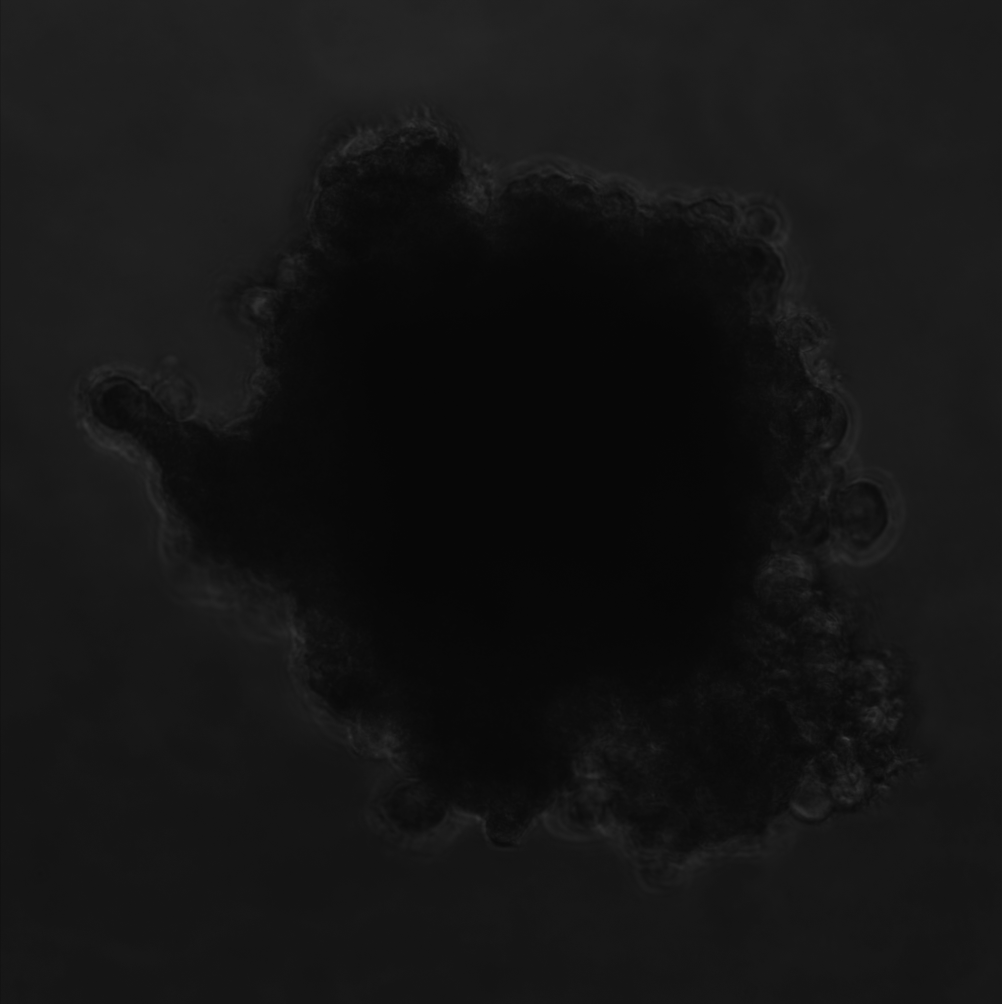
\includegraphics[width=2cm]{figures/result/bn10s_46_image}}
        \subfloat{
\includegraphics[width=2cm]{figures/result/bn10s_46_pred}}
        \subfloat{\includegraphics[width=2cm]{figures/result/bn10s_46_gt}}
    \end{figure}
\end{frame}

%---------------------------------------------------------
\begin{frame}{BN2S - 0.45}
    \begin{figure}[!htb]
        \centering
        \subfloat{\includegraphics[width=2cm]{figures/result/bn2s_04_image}}
        \subfloat{\includegraphics[width=2cm]{figures/result/bn2s_04_pred}}
        \subfloat{\includegraphics[width=2cm]{figures/result/bn2s_04_gt}}\\
        \subfloat{\includegraphics[width=2cm]{figures/result/bn2s_23_image}}
        \subfloat{\includegraphics[width=2cm]{figures/result/bn2s_23_pred}}
        \subfloat{\includegraphics[width=2cm]{figures/result/bn2s_23_gt}}\\
        \subfloat{\includegraphics[width=2cm]{figures/result/bn2s_97_image}}
        \subfloat{\includegraphics[width=2cm]{figures/result/bn2s_97_pred}}
        \subfloat{\includegraphics[width=2cm]{figures/result/bn2s_97_gt}}
    \end{figure}
\end{frame}

%---------------------------------------------------------
\begin{frame}{FL5C - 0.63}
    \begin{figure}[!htb]
        \centering
        \subfloat{\includegraphics[width=3cm]{figures/result/fl5c_01_image}}
        \subfloat{\includegraphics[width=3cm]{figures/result/fl5c_01_pred}}
        \subfloat{\includegraphics[width=3cm]{figures/result/fl5c_01_gt}}\\
        \subfloat{\includegraphics[width=3cm]{figures/result/fl5c_06_image}}
        \subfloat{\includegraphics[width=3cm]{figures/result/fl5c_06_pred}}
        \subfloat{\includegraphics[width=3cm]{figures/result/fl5c_06_gt}}\\
        \subfloat{\includegraphics[width=3cm]{figures/result/fl5c_15_image}}
        \subfloat{\includegraphics[width=3cm]{figures/result/fl5c_15_pred}}
        \subfloat{\includegraphics[width=3cm]{figures/result/fl5c_15_gt}}
    \end{figure}
\end{frame}

%---------------------------------------------------------
\begin{frame}{FL5S - 0.44}
    \begin{figure}[!htb]
        \centering
        \subfloat{\includegraphics[width=3cm]{figures/result/fl5s_08_image}}
        \subfloat{\includegraphics[width=3cm]{figures/result/fl5s_08_pred}}
        \subfloat{\includegraphics[width=3cm]{figures/result/fl5s_08_gt}}\\
        \subfloat{\includegraphics[width=3cm]{figures/result/fl5s_24_image}}
        \subfloat{\includegraphics[width=3cm]{figures/result/fl5s_24_pred}}
        \subfloat{\includegraphics[width=3cm]{figures/result/fl5s_24_gt}}\\
        \subfloat{\includegraphics[width=3cm]{figures/result/fl5s_28_image}}
        \subfloat{\includegraphics[width=3cm]{figures/result/fl5s_28_pred}}
        \subfloat{\includegraphics[width=3cm]{figures/result/fl5s_28_gt}}
    \end{figure}
\end{frame}

%---------------------------------------------------------
\begin{frame}{FN2S - 0.41}
    \begin{figure}[!htb]
    \centering
    \subfloat{\includegraphics[width=2cm]{figures/result/fn2s_04_image}}
    \subfloat{\includegraphics[width=2cm]{figures/result/fn2s_04_pred}}
    \subfloat{\includegraphics[width=2cm]{figures/result/fn2s_04_gt}}\\
    \subfloat{\includegraphics[width=2cm]{figures/result/fn2s_10_image}}
    \subfloat{\includegraphics[width=2cm]{figures/result/fn2s_10_pred}}
    \subfloat{\includegraphics[width=2cm]{figures/result/fn2s_10_gt}}\\
    \subfloat{\includegraphics[width=2cm]{figures/result/fn2s_32_image}}
    \subfloat{\includegraphics[width=2cm]{figures/result/fn2s_32_pred}}
    \subfloat{\includegraphics[width=2cm]{figures/result/fn2s_32_gt}}
    \end{figure}
\end{frame}

%---------------------------------------------------------
\setLayout{horizontal}

\begin{frame}{Comparative Table}
    Metric used: \alert{Mean Jaccard}.
    \begin{table}[]
        \centering
        \setlength{\tabcolsep}{10pt}
        
        {\rowcolors{2}{}{LightGray!10}
            \begin{tabular}{lcccccc}
                Method & BL5S & BN10S & BN2S & FL5C & FL5S & FN2S \\
                \midrule
                Watershed & $0.73$ & $0.64$ & $0.45$ &  $0.63$ & $0.44$ & $0.41$ \\
                U-Net & $0.75^*$ & - & - & $0.93$ & - & -
            \end{tabular}
        }
    \end{table}
\end{frame}

%---------------------------------------------------------
\setLayout{blank}

\begin{frame}{U-Net}
    \begin{figure}[!htb]
        \centering
        \includegraphics[width=13cm]{figures/result/wrong_example}
    \end{figure}
\end{frame}


%---------------------------------------------------------
\begin{frame}{U-Net}
    \begin{figure}[!htb]
        \centering
        \includegraphics[width=13cm]{figures/result/better_example}
    \end{figure}
\end{frame}

\setBGColor{LightPurple}
\section{Final Considerations}

\setLayout{mainpoint}

\begin{frame}[noframenumbering, plain]{}
    \frametitle{Final Considerations}
\end{frame}

\setLayout{vertical}

%---------------------------------------------------------
\begin{frame}{Final Considerations}
    \begin{block}{Found Challenges}
        \begin{itemize}
            \item Handcrafted features lack versatility.
            \item Well annotated spheroids masks.
        \end{itemize}
    \end{block}
    \begin{block}{Our Contribution}
        \begin{itemize}
            \item New unique spheroid dataset.
            \item Self-supervised segmentation for spheroids.
        \end{itemize}
    \end{block}
\end{frame}


%---------------------------------------------------------Slide 8
\setLayout{horizontal}
\begin{frame}
    \frametitle{Sample frame title}
    This is a text in second frame. For the sake of showing an example.
    
    \begin{itemize}
        \item<1-> Text visible on slide 1
        \item<2-> Text visible on slide 2
        \begin{itemize}
            \item text subitem
        \end{itemize}
        \item<3> Text visible on slides 3
        \item<4-> Text visible on slide 4
    \end{itemize}
\end{frame}

%---------------------------------------------------------Slide 9
\setLayout{blank}
\begin{frame}
    
    \centering
    \vspace{2cm}
    
    \textbf{\Huge Thank You}
    
    \ \\
    
    \textbf{}
    \ \\
    
    \text{\footnotesize guilherme.vieira.leite@gmail.com}
    
    \vspace{2cm}
    \begin{figure}
        \centering
        \begin{subfigure}{0.2\textwidth}
            \centering
            \includegraphics[height=1cm]{lib/logos/infw.png}
        \end{subfigure}%
        \qquad 
        \begin{subfigure}{0.2\textwidth}
            \centering
            \includegraphics[height=1cm]{lib/logos/ufgw.png}
        \end{subfigure}
      
    \end{figure}
    
\end{frame}

%---------------------------------------------------------Slide 10
\setLayout{titlepage}
\setBGColor{DarkGray}
\titlepage

\end{document}
